%% 
%% Copyright 2007, 2008, 2009 Elsevier Ltd
%% 
%% This file is part of the 'Elsarticle Bundle'.
%% ---------------------------------------------
%% 
%% It may be distributed under the conditions of the LaTeX Project Public
%% License, either version 1.2 of this license or (at your option) any
%% later version.  The latest version of this license is in
%%    http://www.latex-project.org/lppl.txt
%% and version 1.2 or later is part of all distributions of LaTeX
%% version 1999/12/01 or later.
%% 
%% The list of all files belonging to the 'Elsarticle Bundle' is
%% given in the file `manifest.txt'.
%% 
%% Template article for Elsevier's document class `elsarticle'
%% with harvard style bibliographic references
%% SP 2008/03/01

\documentclass[preprint,12pt,authoryear]{elsarticle}

%% Use the option review to obtain double line spacing
%% \documentclass[authoryear,preprint,review,12pt]{elsarticle}

%% Use the options 1p,twocolumn; 3p; 3p,twocolumn; 5p; or 5p,twocolumn
%% for a journal layout:
%% \documentclass[final,1p,times,authoryear]{elsarticle}
%% \documentclass[final,1p,times,twocolumn,authoryear]{elsarticle}
%% \documentclass[final,3p,times,authoryear]{elsarticle}
%% \documentclass[final,3p,times,twocolumn,authoryear]{elsarticle}
%% \documentclass[final,5p,times,authoryear]{elsarticle}
%% \documentclass[final,5p,times,twocolumn,authoryear]{elsarticle}

%% For including figures, graphicx.sty has been loaded in
%% elsarticle.cls. If you prefer to use the old commands
%% please give \usepackage{epsfig}

%% The amssymb package provides various useful mathematical symbols
\usepackage{amssymb}
%% The amsthm package provides extended theorem environments
%% \usepackage{amsthm}

%% The lineno packages adds line numbers. Start line numbering with
%% \begin{linenumbers}, end it with \end{linenumbers}. Or switch it on
%% for the whole article with \linenumbers.
%% \usepackage{lineno}

\journal{International Journal of Approximate Reasoning}

%%%%%%%%%%%%%%%%%%%%%%%%%%%%%%%%%%%%%%%%%%%%%%%%%%%%%%%%%%%%%%%%%%%%%%%%%%%%%%%
%% Paul's defs
%%%%%%%%%%%%%%%%%%%%%%%%%%%%%%%%%%%%%%%%%%%%%%%%%%%%%%%%%%%%%%%%%%%%%%%%%%%%%%%
\usepackage{bm}
\usepackage{amsthm,amsmath}
\usepackage{subfigure}
%% PHMMs 
\newcommand{\Transition}{\ensuremath{t}}
\newcommand{\Emission}{\ensuremath{e}}

\newcommand{\Sequences}{\ensuremath{S}} 

\newcommand{\Paths}{\ensuremath{\vec{\pi}}}

\newcommand{\Parameters}{\ensuremath{\bm{\Theta}}} 
\newcommand{\TransitionParameters}{\Parameters^{\Transition}} 
\newcommand{\EmissionParameters}{\Parameters^{\Emission}} 

\newcommand{\BoltzmannTransformedParameters}{\ensuremath{\bm{\Omega}}} 
\newcommand{\BoltzmannTransformedTransitionParameters}{\BoltzmannTransformedParameters^{\Transition}} 
\newcommand{\BoltzmannTransformedEmissionParameters}{\BoltzmannTransformedParameters^{\Emission}} 
\newcommand{\boltzmannTransformTemperature}{\ensuremath{\lambda}} 

\newcommand{\NewParameters}{\ensuremath{\tilde{\bm{\Theta}}}}
\newcommand{\NewTransitionParameters}{\NewParameters^{\Transition}} 
\newcommand{\NewEmissionParameters}{\NewParameters^{\Emission}} 

\newcommand{\OtherParameters}{\ensuremath{\bm{\Theta}'}} 

\newcommand{\BWParameters}{\ensuremath{\hat{\bm{\Theta}}}}
\newcommand{\BWTransitionParameters}{\BWParameters^{\Transition}} 
\newcommand{\BWEmissionParameters}{\BWParameters^{\Emission}} 

\newcommand{\ParametersSubset}{\ensuremath{\bm{\Phi}}}
\newcommand{\TransitionParametersSubset}{\ParametersSubset^{\Transition}} \newcommand{\EmissionParametersSubset}{\ParametersSubset^{\Emission}} 

\newcommand{\ParametersSubsetComplement}{\ensuremath{\bm{\Psi}}}
\newcommand{\TransitionParametersSubsetComplement}{\ParametersSubsetComplement^{\Transition}}
\newcommand{\EmissionParametersSubsetComplement}{\ParametersSubsetComplement^{\Emission}} 

\newcommand{\NewParametersSubset}{\ensuremath{\tilde{\bm{\Phi}}}}
\newcommand{\NewTransitionParametersSubset}{\NewParametersSubset^{\Transition}} 
\newcommand{\NewEmissionParametersSubset}{\NewParametersSubset^{\Emission}} 

\newcommand{\CBWParametersSubset}{\ensuremath{\hat{\bm{\Phi}}}}
\newcommand{\CBWTransitionParametersSubset}{\CBWParametersSubset^{\Transition}} \newcommand{\CBWEmissionParametersSubset}{\CBWParametersSubset^{\Emission}} 

\newcommand{\OtherParametersSubset}{\ensuremath{\bm{\Phi}'}}

\newcommand{\Counts}{\ensuremath{C}} 
\newcommand{\TransitionCounts}{\Counts^{\Transition}}
\newcommand{\EmissionCounts}{\Counts^{\Emission}}

\newcommand{\ExpectedCounts}{\ensuremath{N}} 
\newcommand{\ExpectedTransitionCounts}{\ExpectedCounts^{\Transition}}
\newcommand{\ExpectedEmissionCounts}{\ExpectedCounts^{\Emission}}

\newcommand{\TotalExpectedCounts}{\ensuremath{Z}} 
\newcommand{\TotalExpectedTransitionCounts}{\TotalExpectedCounts^{\Transition}}
\newcommand{\TotalExpectedEmissionCounts}{\TotalExpectedCounts^{\Emission}}

\newcommand{\transition}{\ensuremath{\bm{t}}}
\newcommand{\emission}{\ensuremath{\bm{e}}}
\newcommand{\parameter}{\ensuremath{\bm{\theta}}}
\newcommand{\parametersSubsetParameter}{\ensuremath{\bm{\phi}}}
\newcommand{\boltzmannTransformedParameter}{\ensuremath{\bm{\omega}}}

\newcommand{\transitionValue}{\ensuremath{t}}
\newcommand{\emissionValue}{\ensuremath{e}}
\newcommand{\parameterValue}{\ensuremath{\theta}}
\newcommand{\boltzmannTransformedParameterValue}{\ensuremath{\omega}}

\newcommand{\sequenceIndex}{\ensuremath{m}}
\newcommand{\maxSequenceIndex}{\ensuremath{M}}
\newcommand{\residueIndex}{\ensuremath{j}}
\newcommand{\maxResidueIndex}{\ensuremath{J}}
\newcommand{\datum}{\ensuremath{d}}
\newcommand{\residue}{\ensuremath{r}}
\newcommand{\residueToDatumMap}{\ensuremath{l}}
%\newcommand{\sequence}{\ensuremath{s}}
\newcommand{\hiddenState}{\ensuremath{h}}
\newcommand{\pathComponent}{\ensuremath{\pi}}

\newcommand{\Time}{\ensuremath{\tau}}
\newcommand{\maxTime}{\ensuremath{K}}
\newcommand{\States}{\ensuremath{\mathcal{S}}}
\newcommand{\state}{\ensuremath{s}}
\newcommand{\maxState}{\ensuremath{S}}
\newcommand{\PathComponents}{\ensuremath{\mathcal{P}}}

\newcommand{\bwTransition}{\ensuremath{\hat{\transition}}}
\newcommand{\bwEmission}{\ensuremath{\hat{\emission}}}
\newcommand{\bwParameterValue}{\ensuremath{\hat{\parameterValue}}}

\newcommand{\qaStepSize}{\ensuremath{\eta}}

\newcommand{\otherTransition}{\ensuremath{\transition '}}
\newcommand{\otherEmission}{\ensuremath{\emission '}}
\newcommand{\otherParameter}{\ensuremath{\parameter '}}
\newcommand{\otherParameterValue}{\ensuremath{\parameterValue '}}

\newcommand{\multinomial}{\ensuremath{m}}

%\newcommand{\Substates}{\ensuremath{\mathbb{B}}}
%\newcommand{\substate}{\ensuremath{b}}
\newcommand{\substateMatch}{\ensuremath{\mathbb{M}}}
\newcommand{\substateInsertion}{\ensuremath{\mathbb{I}}}
\newcommand{\substateDeletion}{\ensuremath{\mathbb{D}}}
\newcommand{\substateBegin}{\ensuremath{\mathbb{B}}}
\newcommand{\substateTerminal}{\ensuremath{\mathbb{T}}}

\newcommand{\HMMtransitionLaw}{\ensuremath{t}}
\newcommand{\HMMemissionLaw}{\ensuremath{e}}

%\newcommand{\PHMMtransitionLaw}{\ensuremath{t}}
%\newcommand{\PHMMemissionLaw}{\ensuremath{e}}
\newcommand{\insertionEmissionLaw}{\ensuremath{e_{\substateInsertion}}}

\newcommand{\forward}{\ensuremath{\alpha}}
\newcommand{\backward}{\ensuremath{\beta}}

%%%%%%%%%%%%%%%%%%%%%%%%%%%%%%%%%%%%%%%%%%%%%%%%%%%%%%%%%%%%%%%%%%%%%%%%%%%%%%%
%% Probability
\newcommand{\Prob}{\ensuremath{\mathbb P}} 
\newcommand{\ExpectedValue}{\ensuremath{\mathbb E}} 
\newcommand{\Var}{\ensuremath{\hbox{Var}}} 

%% (Probability) Distributions
\newcommand{\Edist}{\ensuremath{\mathcal{E}\hbox{xpo}}} 
\newcommand{\Ndist}{\ensuremath{\mathcal N}} 
\newcommand{\Udist}{\ensuremath{\mathcal U}} 
\newcommand{\Gdist}{\ensuremath{\mathcal{G}\hbox{amma}}}
\newcommand{\Pdist}{\ensuremath{\mathcal{P}\hbox{ois}}}
\newcommand{\Bdist}{\ensuremath{\mathcal{B}\hbox{eta}}}

%% (Statistical) Independence
\newcommand\independent{\protect\mathpalette{\protect\independenT}{\perp}}
\def\independenT#1#2{\mathrel{\rlap{$#1#2$}\mkern2mu{#1#2}}}

%% Asymptotics
\newcommand{\dArrow}{\ensuremath{\stackrel{d}{\longrightarrow}}} 
\newcommand{\dEquals}{\ensuremath{\stackrel{d}{=}}} 
\newcommand{\pArrow}{\ensuremath{\stackrel{p}{\longrightarrow}}} 
\newcommand{\asArrow}{\ensuremath{\stackrel{a.s.}{\longrightarrow}}} 
\newcommand{\rArrow}{\ensuremath{\stackrel{r}{\longrightarrow}}} 
\newcommand{\as}{\ensuremath{\hspace{1em}\hbox{ as }\hspace{1em}}}
\newcommand{\asni}{\ensuremath{\hspace{1em}\hbox{ as }
	\hspace{1em}n\rightarrow\infty}}

%% Argmax!
\newcommand{\argmax}{\operatornamewithlimits{argmax}}

%% Derivatives
\newcommand{\ppt}{\frac{\partial}{\partial\theta}} 
\newcommand{\ddt}{\frac{d}{d\theta}} 

%% Complexity
\newcommand{\BigO}{\ensuremath{\hbox{O}}} 

%% Dempster-Shafer
\newcommand{\Mass}{\ensuremath{\hbox{Mass}}} 
\newcommand{\Bel}{\ensuremath{\hbox{Bel}}} 
\newcommand{\Plaus}{\ensuremath{\hbox{Plaus}}} 
\newcommand{\Comm}{\ensuremath{\hbox{Comm}}} 

%% Spacing
\newcommand{\n}{\hspace{.5em}} 
\newcommand{\m}{\hspace{1em}} 
\newcommand{\mm}{\hspace{2em}} 
\newcommand{\mmm}{\hspace{3em}} 
\newcommand{\ignore}[1]{}
%%%%%%%%%%%%%%%%%%%%%%%%%%%%%%%%%%%%%%%%%%%%%%%%%%%%%%%%%%%%%%%%%%%%%%%%%%%%%%%
%% END Paul's defs
%%%%%%%%%%%%%%%%%%%%%%%%%%%%%%%%%%%%%%%%%%%%%%%%%%%%%%%%%%%%%%%%%%%%%%%%%%%%%%%

\begin{document}

\begin{frontmatter}

%% Title, authors and addresses

%% use the tnoteref command within \title for footnotes;
%% use the tnotetext command for theassociated footnote;
%% use the fnref command within \author or \address for footnotes;
%% use the fntext command for theassociated footnote;
%% use the corref command within \author for corresponding author footnotes;
%% use the cortext command for theassociated footnote;
%% use the ead command for the email address,
%% and the form \ead[url] for the home page:
\title{The Conditional Quadratic Ascent Procedure for Maximum-A-Posteriori Parameter Estimation of Profile Hidden Markov Models, with an Application to HIV-1 Founder Identification}
%%\tnotetext[label1]{}
\author{Paul T. Edlefsen\corref{cor1}}
%% \ead[url]{home page}
%%\fntext[label2]{}
%%\cortext[cor1]{\ead{pedlefse@fredhutch.org}}
\cortext[cor1]{\ead{pedlefse@fredhutch.org}}
\address{Fred Hutchinson Cancer Research Center}
%% \fntext[label3]{}

%% \title{}

%% use optional labels to link authors explicitly to addresses:
%% \author[label1,label2]{}
%% \address[label1]{}
%% \address[label2]{}

%%\author{}

%%\address{}

\begin{abstract}
  Previous studies have shown that a conditional maximization variant
  of the Baum-Welch algorithm improves parameter estimation for the
  profile hidden Markov models (PHMMs) widely used in genomic sequence
  analysis.  In this article we introduce an alternative conditional
  maximization approach that directly maximizes the conditional
  likelihood through gradient ascent, combining the Baldi-Chauvin
  gradient determination with a successive parabolic line search.
  Through simulation studies we show that this new method outperforms
  not only its non-conditional variant but also both Baum-Welch and
  Conditional Baum-Welch.  We measure performance on both training
  data and held-out validation data, and the new method performs
  especially well on validation data as compared with these standard
  approaches, and especially well when there are few sequences available for parameter estimation.  We also demonstrate an application of the new approach
  to estimating the parameters of profile hidden Markov models of
  HIV-1 data sampled in acute infection, when single founders of
  infection are expected to follow the star-like phylogeny implied by
  the PHMM. By using a simple approach to identify multiple founders of infection as violations of that model assumption, we present a first effort towards fully automated HIV-1 founder detection.
% We
%   also show that the previously-reported Dynamic Model Surgery
%   algorithm is unnecessary when the initial model parameters are chosen to
%   be nearly evenly distributed across the DNA or amino acid residues
%   at each position of the model.
\end{abstract}

\begin{keyword}
profile hidden Markov model \sep genomic sequence alignment \sep statistical inference \sep HIV \sep CBW \sep CQA

%% keywords here, in the form: keyword \sep keyword

%% PACS codes here, in the form: \PACS code \sep code

%% MSC codes here, in the form: \MSC code \sep code
%% or \MSC[2008] code \sep code (2000 is the default)

\end{keyword}

\end{frontmatter}

%% \linenumbers

%% main text
\section{Introduction}
\label{Introduction}
We previously introduced a new algorithm for estimating parameters
of Hidden Markov Models (HMMs).  The algorithm, Conditional
Baum-Welch, is a variant of the Baum-Welch algorithm
\citep{Baum:1972}.  Baum-Welch is a computationally efficient
expectation-maximization (EM) algorithm \citep{DempsterEM:1977,
  scott:2002} for HMMs.  Conditional Baum-Welch is as efficient as
Baum-Welch for HMMs that satisfy a sparseness condition.  One such HMM
is the profile hidden Markov model (Profile HMM, or PHMM) \citep{Rabiner:1989, Durbin}, commonly used to
model families of related protein sequences.  Both the Baum-Welch and
the Conditional Baum-Welch algorithms converge to a local optimum.  There is no guarantee that the optimum is
global, and in the context of Profile HMMs, the landscape is
sufficiently rugged that premature convergence to local optima is
often a problem.  We previously showed Profile HMM results demonstrating that
the Conditional Baum-Welch algorithm converges to higher optima than
the standard (``Unconditional'') Baum-Welch under a range of conditions \citep{edlefsen2010transposon}.  We also introduced the
Dynamic Model Surgery algorithm, which further improves both
Baum-Welch and Conditional Baum-Welch by detecting and escaping traps
in the rugged optimization landscape.

In this article we introduce an alternative method, Quadratic Ascent, with both
conditional and unconditional variants.  Like the Conditional
Baum-Welch algorithm, the conditional variant of this new method
employs a ``rotated'' forward-backward procedure that takes advantage
of the sparseness of the transition matrix of the underlying Markov
chain to isolate and conditionally update the parameters of the model.
Rather than employ the Baum-Welch Expectation Maximization procedure, which maximizes the expected value of the negative
log-likelihood, the Quadratic Ascent algorithm directly ascends the
likelihood by moving the parameters in the direction of steepest ascent.

The essential insight behind these conditional maximization approaches
was serendipitously discovered.  Although the Baum-Welch algorithm is
typically described and implemented using recursions (``forward'' and
``backward'', described below) in time, in some instances it can be
implemented using recursions in space rather than time.  Essentially
these recursions calculate function values in the cells of a matrix, and the Baum-Welch forward-backward algorithm is typically described as calculating each column of the matrix as a (linear) function of the previous column.  With the Profile HMM, the algorithm can be just as well described as calculating these values row-by-row, with each row calculated as a linear function of the previous row.  Since each row of the matrix corresponds to a state of the model, this row-wise orientation inspires conditional maximization algorithms that modify state-specific parameters row-by-row, interweaved with the forward-backward calculations.

Improving parameter estimation for hidden Markov models is worthwhile
wherever they are applied, but this research is particularly motivated
by the need for a better approach to parameterizing Profile HMMs.
While Profile HMMs are widely used to model protein sequence families,
their use for modeling DNA sequence families has been slow to develop.
In fact, the two major Profile HMM software packages, HMMer
\citep{eddy:1992} and SAM \citep{SAM,hughey:1996}, originally supported
DNA sequences but, until recently, both retained only token support, with all development
effort focused on proteins.  The latest version of HMMer \citep[version 3.1:][]{HMMerUsersGuide3.1,FinnHMMer3}, reintroduces support for DNA search with nhmmer \citep{Wheeler2013}, but this iteration of HMMer does not support building profiles from unaligned sequences, despite the origin of the HMMer package as an implementation of the Baum-Welch algorithm \citep{Durbin}.  It turns out that Baum-Welch is 
particularly prone to get stuck in local optima when the sequences are
composed of only the four nucleotide residues of DNA, as opposed to
the twenty amino acid residues of protein sequences.  Furthermore,
protein sequence alignment approaches that employ Profile HMMs
for remote homology detection are prone to fail when the sequences are
diverged beyond the ability of the Baum-Welch algorithm \citep{kececioglu2010aligning}.  Improving
parameter estimation for Profile HMMs in both protein and nucleic acid
contexts has great potential impact in medicine and
biology, and wherever improved genomic sequence alignment (and statistical uncertainty assessment therein) is valued.

The Profile HMM approach is a way to simultaneously account for all
possible multiple alignments.  The common reliance by bioinformatics
projects on single multiple alignments is problematic, since different
multiple alignments result in different ``downstream'' analyses.  For
instance it is typical for probabilistic phylogenetic studies to
depend on a single multiple alignment, with no account made for the
error introduced by the variation in alignments.  This problem has
recently received increased attention
\citep[e.g. see][]{Lunter:2008fj,Wong:2008wj}.  The Profile HMM can be
viewed as a model of the joint probability distribution of alignments
and sequences.  Profile HMMs have been proposed for use as alternatives to
progressive multiple alignment algorithms \citep[e.g.][]{eddy:1995}, but since they
represent a distribution of multiple alignments, they can als be used in
more sophisticated ways, such as for drawing random alignments, or for
evaluating relative probabilities of different alignments.
 
%We were directed to Profile HMMs through an earlier effort to improve the transposon modeling software RepeatMasker \citep{RepeatMasker, Jurka:2005}.  Transposons are virus-like elements that duplicate themselves in the genome.  They are so ubiquitous that biologists often prefer to remove them before doing genomic analyses.  We argue in \cite{edlefsen2010transposon} that there are many reasons to desire improved transposon models and identification techniques, apart from ``masking.''  Since most transposons are no longer active, they undergo gradual degradation over time.  At least 45\% of the human genome is composed of the remnants of once-active transposable elements \citep{NatureHumanGenome:2001}, most of which have been degraded by mutations and gaps.  There are probably many that have degraded beyond recognition by the current techniques \citep{Lerat:2007,Medstrand:2002}.

% Until recently, the RepeatMasker software relied on multiple alignments of
% known transposon elements to create the ``consensus'' sequences used
% to search for new elements.  Many transposon families are so highly
% diverged that the various available multiple alignment software
% programs generate very different ad-hoc alignments, resulting in
% different consensus models.  We showed in \cite{edlefsen2010transposon}
% that Profile HMMs are a viable alternative with desirable features,
% and that the Conditional Baum-Welch algorithm provides an essential
% improvement over Baum-Welch for this problem. In the interim, the HMMer software was rewritten to use Profile HMMs, a development that led to marked improvements in transposon identification \citep{TravissBenchmarksPaper}.  This, together with the new support for DNA search \citep{Wheeler2013,HMMerUsersGuide3.1} also led to the development of the first database of Profile Hidden Markov models for DNA sequence families, DFAM \citep{DFAM}.  However, at this time the models in DFAM are constructed from hand-curated alignments because HMMer does not implement Baum-Welch or any other method for parameter estimation from unaligned sequences.
% 
% While presently DFAM supports only models of endogenous virus families (transposons), we aim to contribute models of 

Here we aim to apply Profile HMMs to modeling and aligning HIV-1, a highly variable exogenous viral genome that is notoriously difficult to align.  While automated alignment software exists that is specifically tailored to HIV-1 \citep{Gaschen01052001}, in practice HIV-1 multiple alignment requires skilled manual labor.  A critical shortcoming of this manual approach, apart from its irreproducibility, is that downstream analyses relying on HIV-1 alignments inevitably fail to account for the uncertainty.  For example, Bayesian phylogenetic models misrepresent posterior credibility when they condition on a single input alignment.

%%% TODO: Get refs about how HIV is hard to align.

Full-scale implementation of Profile HMMs for modeling viruses and
other highly diverged genomic sequence families has been hindered by
the relative instability of the available estimation procedures.  Unfortunately we found that this is the case even when employing the Dynamic Model Surgery (DMS) procedure that we previously introduced, without which even the Conditional Baum-Welch algorithm is insufficient to escape the many optimization traps (inescapable local
maxima) found in the parameter landscape.  We are pleased to report
that with a more careful choice of starting parameters, all of these
search algorithms (Baum-Welch, Conditional Baum-Welch, and the new
Quadratic Ascent algorithms) can be made to achieve optima in the
absence of DMS otherwise accessible only when used with DMS.
Furthermore, the Conditional Quadratic Ascent (CQA) algorithm achieves
maxima comparable and in some cases superior to those achieved by Conditional
Baum-Welch, and in conditions relevant to HIV-1 modeling the parameters estimated by (Conditional) Quadratic
Ascent are more similar to the simulated true parameters than those
estimated by (Conditional) Baum-Welch, and results on cross-validation
sets are consistently superior with the new approach.

The remainder of this article is organized as follows.  We first
describe the Profile HMM and briefly review the Baum-Welch and Conditional Baum-Welch
algorithms.  We then introduce and describe the new Quadratic Ascent
algorithm through its conditional variant.  In the Results section, we
show through simulation studies the degree of improvement conferred by
the new algorithm variants in the context of both amino acid sequence
families and DNA sequence families across a range of simulation
conditions. We also demonstrate an application of the new approach to
estimating the parameters of profile hidden Markov models of HIV-1
data sampled in acute infection, when single founders of infection are
expected to follow the ``star-like'' phylogeny implied by the PHMM, using a simple idea to detect multiple founders of infection as violations of
that model assumption.  We conclude with a discussion of
the implications of these findings and directions for future study.

\section{Baum-Welch}
\subsection{The Hidden Markov Model}
The hidden Markov model (HMM) is a statistical model that has been widely applied across an array of disciplines, including notably time series analysis and natural language processing, and biological sequence alignment \citep{Rabiner:1989,Churchill:1989eu,Baldi:1994, Krogh:1994lr,Liu:1999}. An HMM with parameters $\Parameters$ describes the joint distribution $\Prob( \vec{\datum}, \vec{\hiddenState} | \Parameters )$ of a vector of observed data $\datum_{1}, \dots, \datum_{\maxTime}$ and a vector of the corresponding hidden data $\hiddenState_{1}, \dots, \hiddenState_{\maxTime}$. Expressed in terms of a time series, an HMMs models the distribution of an observation $\datum_{\Time}$ at time $\Time \in 1..\maxTime$ as conditionally independent from observations at other times, given the latent state $\hiddenState_{\Time}$ of a Markov chain at time $\Time$:
\begin{equation}\label{cbw_eq:HMM_EmissionLaw}
\datum_{\Time} \sim \HMMemissionLaw_{\Time}( \cdot | \hiddenState_{\Time} ) \hbox{,}
\end{equation}
\begin{equation}\label{cbw_eq:HMM_TransitionLaw}
\hiddenState_{\Time} \sim \HMMtransitionLaw_{\Time}( \cdot | \hiddenState_{\Time - 1} ) \hbox{,}
\end{equation}
where $\HMMemissionLaw_{\Time}( \cdot | \hiddenState_{\Time} )$ is the ``emission'' distribution of the observations and $\HMMtransitionLaw_{\Time}( \cdot | \hiddenState_{\Time - 1} )$ as the ``transition'' distribution of the underlying Markov process.  Figure~\ref{cbw_fig:HMM} depicts the dependence structure of a generic HMM.

\begin{figure}[htp]
\centering
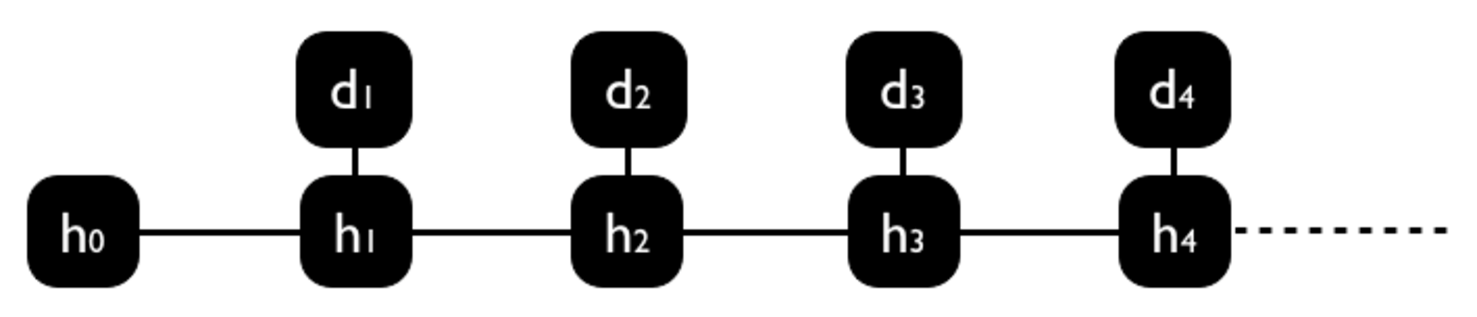
\includegraphics[scale=.5]{HMM.pdf} \\
 \caption{\textbf{The hidden Markov model.} The state of an unobserved Markov chain $\hiddenState_{\Time}$ evolves over time $\Time$ according to transition kernel $\HMMtransitionLaw_{\Time}( \cdot | \hiddenState_{\Time - 1} )$.  At each time the observed datum  $\datum_{\Time}$ is distributed according to the ``emission'' distribution $\HMMemissionLaw_{\Time}( \cdot | \hiddenState_{\Time} )$, which depends on the current state of the hidden Markov chain. [Figure~1 from \cite{edlefsen2010transposon}, reproduced with permission.]}
 \label{cbw_fig:HMM}
\end{figure}

The Profile HMM is a special case of this general approach, adapted for use in modeling a genomic sequence alignment \citep{Durbin}.  Here, the sequence residues are the observed data $\vec{\datum}$, with each time $\Time$ associated with exactly one of the observed residues ($\datum_{\Time}$).  The hidden states of the Markov chain represent the positions of an ancestral reference sequence.  Due to the processes of evolution (mutation and insertion/deletion), the correspondence between the ancestral and observed positions is obscured; its resolution constitutes a pairwise sequence alignment between the homologous pair (ancestor, decendant). Figure~\ref{cbw_fig:Plan7} depicts the Profile HMM.

\begin{figure}[htp]
\centering
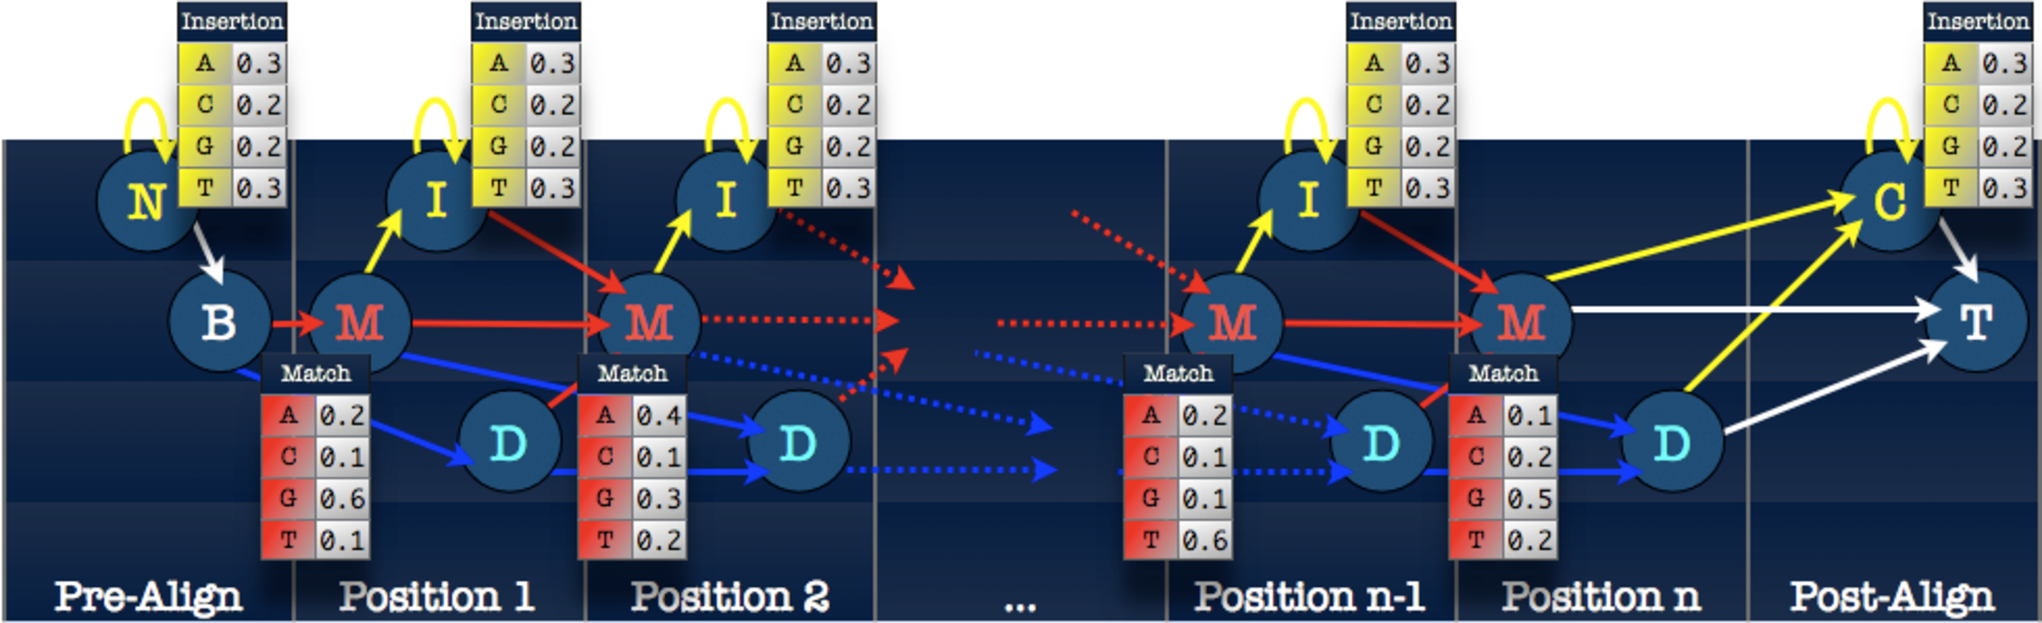
\includegraphics[scale=.445]{Plan7.pdf} \\
 \caption{\textbf{The states of the Profile HMM.} There are $3n + 4$ states for a Profile HMM representing a sequence family with $n$ ancestral positions.  Each internal position has three associated states: Match, Insertion, and Deletion.  Additional states represent flanking insertions.  All match and insertion states have an associated emission distribution, which is multinomial over the allowed residues.  The insertion emission distributions typically reflect the background residue frequencies, while the match distributions are position-specific. [Figure~2 from \cite{edlefsen2010transposon}, reproduced with permission.]}
  \label{cbw_fig:Plan7}
\end{figure}

\subsection{Baum-Welch and the forward and backward values}
The transition and emission parameters of a Hidden Markov Model are generally estimable using a polynomial-time algorithm, Baum-Welch, which can be expressed as an instance of the expectation maximization (EM) algorithm for maximum-likelihood or maximum a-posteriori parameter estimation \citep{Baum:1972, DempsterEM:1977, Rabiner:1989}.  The algorithm uses dynamic programming to calculate ``forward'' values $\forward_{\Time}( \hiddenState_{\Time} ) = \Prob( \datum^{\Time}, \hiddenState_{\Time} | \Parameters )$, where $\datum^{\Time}$ represents the initial $\Time$ residues of observed sequence $\vec{\datum}$.

The probability of the sequence $\vec{\datum}$ given the parameterized model is easily calculated from the forward value, since
\begin{equation}\label{cbw_eq:ForwardLikelihood}
\begin{split}
\Prob( \vec{\datum} | \Parameters )
 & = \Prob( \datum^{\maxTime} | \Parameters ) \\
 & = \sum_{\hiddenState_{\maxTime} \in \States}{ \Prob( \datum^{\maxTime}, \hiddenState_{\maxTime} | \Parameters ) } \\
 & = \sum_{\hiddenState_{\maxTime} \in \States}{ \forward_{\maxTime}( \hiddenState_{\maxTime} ) } \hbox{,}
\end{split}
\end{equation}
where $\States$ is the state space of the Markov chain, and $\maxTime = |\vec{\datum}|$ is the length of the sequence $\vec{\datum}$.

The dynamic programming recursion for computing $\forward_{\Time}$ as a function of $\forward_{\Time - 1}$ follows from the conditional independence assumptions of the Markov chain underlying the HMM:
\begin{equation}\label{cbw_eq:forwardByTime}
\forward_{\Time}( \hiddenState_{\Time} )
 = \sum_{\hiddenState_{\Time - 1} \in \States}{ \forward_{\Time - 1}( \hiddenState_{\Time - 1 } ) \HMMtransitionLaw( \hiddenState_{\Time} | \hiddenState_{\Time - 1} ) \HMMemissionLaw( \datum_{\Time} | \hiddenState_{\Time} ) } \hbox{.}
\end{equation}

The ``backward'' value $\backward_{\Time}( \hiddenState_{\Time} ) = \Prob( \datum^{-\Time} | \hiddenState_{\Time}, \Parameters )$ is the conditional distribution of the remaining $\maxTime - \Time$ components of $\vec{\datum}$ (after $\datum_{\Time}$), which we denote by $\datum^{-\Time}$, given the state $\hiddenState_{\Time}$ at time $\Time$.  The recursion for calculating the backward value is similar to that of the forward value, only in reverse:
\begin{equation}\label{cbw_eq:backwardByTime}
\backward_{\Time}( \hiddenState_{\Time} )
 = \sum_{\hiddenState_{\Time + 1} \in \States}{ \backward_{\Time + 1}( \hiddenState_{\Time + 1 } ) \HMMtransitionLaw( \hiddenState_{\Time + 1} | \hiddenState_{\Time} ) \HMMemissionLaw( \datum_{\Time + 1} | \hiddenState_{\Time + 1} ) } \hbox{.}
\end{equation}

The forward or the backward values can be used to efficiently calculate the likelihood function (Equation~\ref{cbw_eq:ForwardLikelihood}).  The forward and backward values together yield the conditional distribution of the hidden state $\hiddenState_{\Time}$ given the observed sequence $\vec{\datum}$, since
\begin{equation*}
\begin{split}
\Prob( \hiddenState_{\Time} | \vec{\datum}, \Parameters )
 &= \frac{ \Prob( \hiddenState_{\Time}, \vec{\datum} | \Parameters ) }{\Prob( \vec{\datum} | \Parameters ) } \\
 &= \frac{ \forward_{\Time}( \hiddenState_{\Time} ) \backward_{\Time}( \hiddenState_{\Time} ) }{\Prob( \vec{\datum} | \Parameters ) } \hbox{.}
\end{split}
\end{equation*}
In a Bayesian context this can be used to compute the posterior probability that the HMM ``emitted'' the $\Time^{th}$ residue of sequence $\vec{\datum}$ from state $\hiddenState_{\Time}$. Assuming a degenerate prior, the joint posterior distribution of $\hiddenState_{\Time-1}$ and $\hiddenState_{\Time}$ is
\begin{equation*}
\begin{split}
\Prob( \hiddenState_{\Time-1}, \hiddenState_{\Time} | \vec{\datum}, \Parameters )
 &= \frac{ \Prob( \hiddenState_{\Time-1}, \hiddenState_{\Time}, \vec{\datum} | \Parameters ) }{\Prob( \vec{\datum} | \Parameters ) } \\
 &= \frac{ \forward_{\Time-1}( \hiddenState_{\Time} ) \HMMtransitionLaw( \hiddenState_{\Time} | \hiddenState_{\Time - 1} ) \HMMemissionLaw( \datum_{\Time} | \hiddenState_{\Time} ) \backward_{\Time}( \hiddenState_{\Time} ) }{ \Prob( \vec{\datum} | \Parameters ) } \hbox{.}
\end{split}
\end{equation*}

The Baum-Welch procedure iteratively replaces the parameters $\EmissionParameters$ of the ``emission'' distribution $\HMMemissionLaw$ and the parameters $\TransitionParameters$ of the ``transition'' distribution $\HMMtransitionLaw$ such that each parameter is proportional to the average (over all of the observed sequences) of the expected number of uses of the corresponding emission (or transition). We have previously shown that a conditional maximization variant of Baum-Welch (Conditional Baum-Welch) converges to better local optima than the Baum-Welch algorithm in the context of profile hidden Markov models \citep{edlefsen2010transposon}.  As EM algorithms, both Baum-Welch and Conditional Baum-Welch achieve maximization indirectly by maximizing an auxiliary function that is guaranteed to lie below the objective function (an approach known generally as Minorization/Maximization, or MM \citep{Hunter:2004}).  This auxiliary function is the so-called ``Q function'' of the EM algorithm.  Here we introduce an alternative procedure that uses the same ``rotated orientation'' approach employed by Conditional Baum-Welch, but which employs a form of gradient ascent to directly maximize the posterior probability of the data.

\section{Conditional Baum-Welch and the ``rotated'' orientation}
We now briefly describe the logic of the ``rotated'' orientation used by both the Conditional Baum-Welch (CBW) algorithm and the CQA algorithm.  We have shown through simulation studies that CBW is often able to escape the local optima that trap the Baum-Welch (UBW) algorithm.  CBW depends on the same update procedure as Baum-Welch, but iteratively applies this procedure to conditional parameter distributions rather than to the complete joint likelihood/posterior.  As Baum-Welch is an example of the EM algorithm, Conditional Baum-Welch is an example of a multi-cycle ECM (Expectation Conditional Maximization) algorithm \citep{MengECM:1993,meng:1997aof}.  Like Baum-Welch, CBW is guaranteed to increase the likelihood.% (see the Appendix for a proof).

The CBW and CQA algorithms separately update the parameters associated with each model position (cf. Figure~\ref{cbw_fig:Plan7}), holding fixed the values of the other parameters.  In CBW this is iterated with standard Baum-Welch updates of parameters that apply to multiple states.   See \cite{edlefsen2010transposon} for further details.

\begin{figure}[htp]
\centering
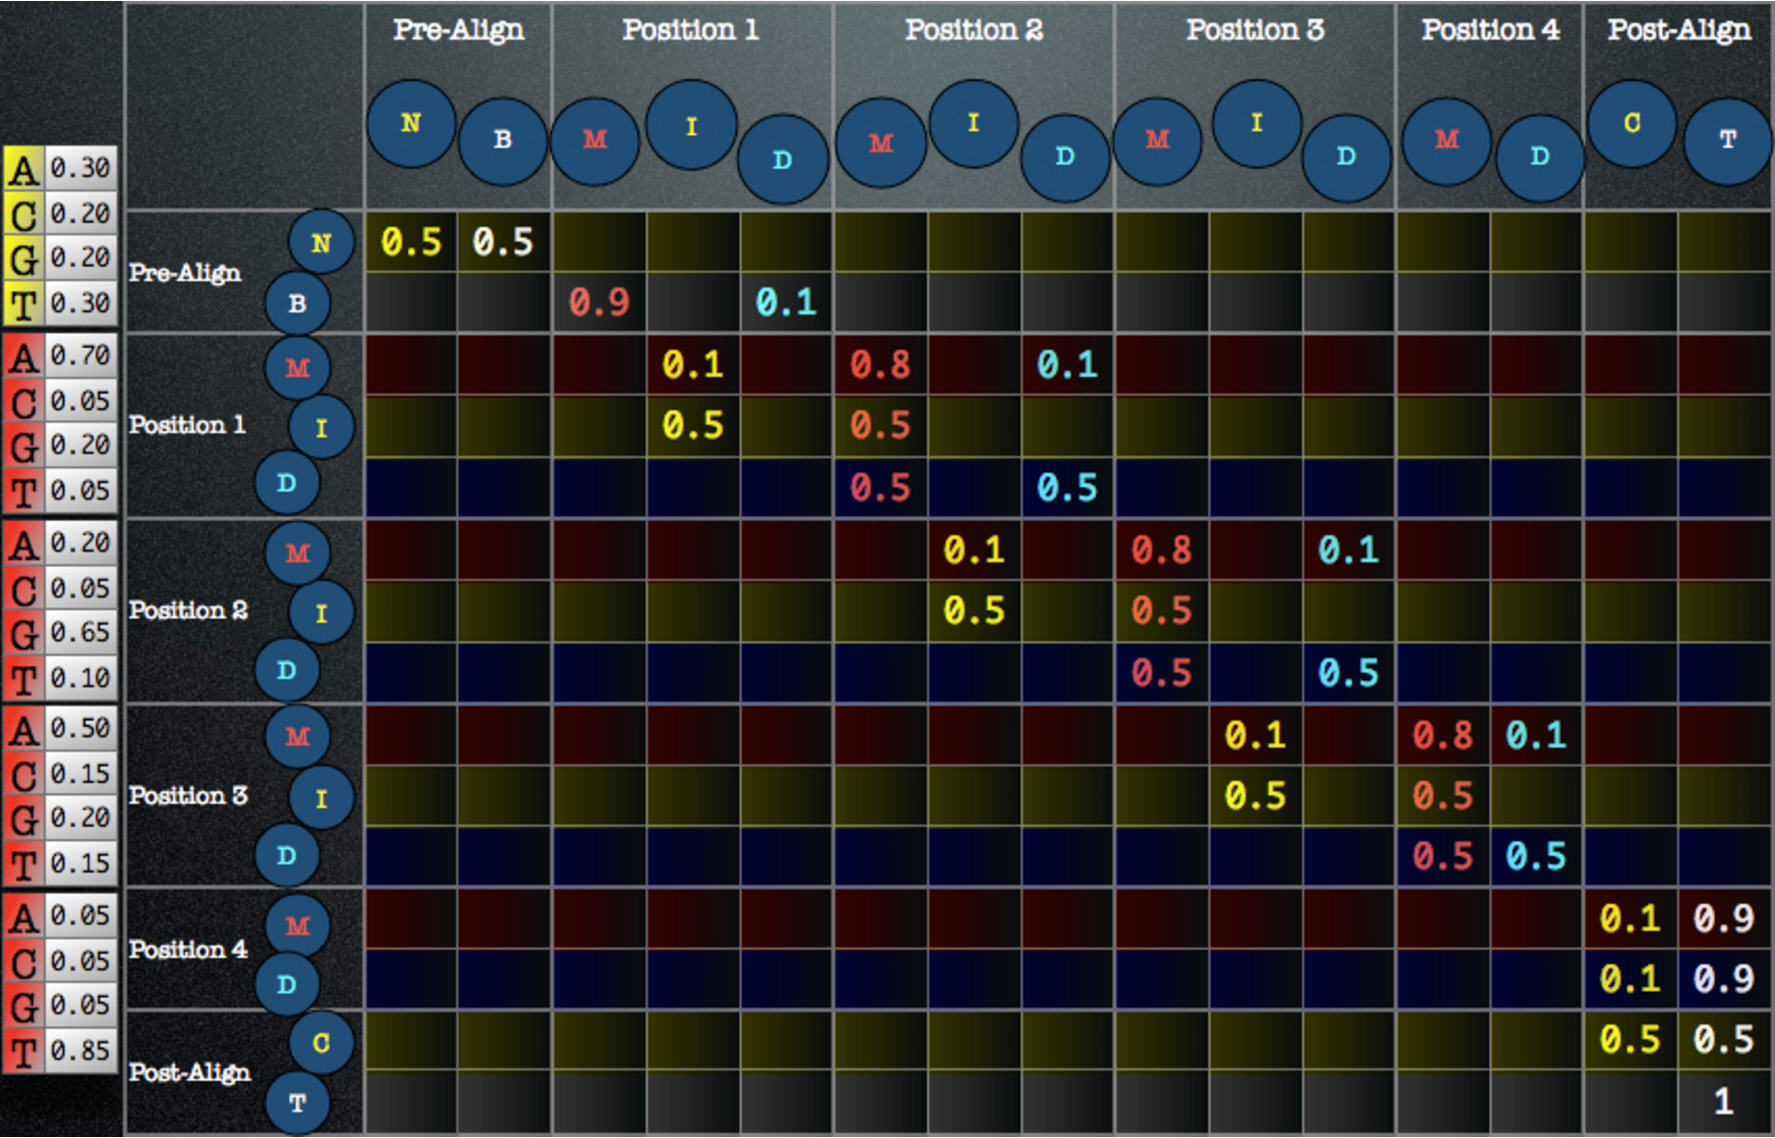
\includegraphics[scale=.5]{Plan7Parameters.pdf} \\
 \caption{\textbf{The parameters of a four-position Profile HMM.} There are $16$ states for a Profile HMM representing a sequence family with $4$ ancestral positions.  The transition parameters $\TransitionParameters$ are represented as a transition matrix among the states.  Blank elements of the transition matrix represent transitions disallowed by the model.  Note that all transitions are relatively local, and the matrix is relatively diagonal.  The emission parameters $\EmissionParameters$ are depicted along the left edge of the transition matrix.  Each position has its own multinomial Match emission distribution, and all positions share an Insertion emission distribution.  The numbers given are examples; the BW, CBW, and CQA algorithms find values that are maxima in the likelihood (or posterior probability) landscape for a set of training sequences.}
  \label{cbw_fig:Plan7Parameters}
\end{figure}

For CBW and CQA to be as efficient as BW, the transition probability matrix of the underlying Markov chain must be relatively sparse and relatively diagonal.  In particular, there must exist an ordering of the states $\States = \state_1, \dots, \state_{\maxState}$ such that the probability $t(s_i,s_j)$ of transitioning from state $i$ to state $j$ is zero unless $j \geq i$ and $(j - i) \leq k$ for some fixed small constant $k$.  As an example, consider the transition matrix depicted in Figure~\ref{cbw_fig:Plan7Parameters}, which is an example of a transition matrix for a four-position Profile HMM.  For the Profile HMM model, the condition is satisfied with $k = 5$ (from a Match state at one position to the Deletion state at the subsequent position).

When this condition is satisfied, the forward and backward dynamic programming recursions can proceed state-by-state rather than time-by-time.  That is, instead of computing the forward values $\forward_{\Time}( \hiddenState_{\Time} )$ for time $\Time$ as a function of the forward values for all states at the previous time (as in Equation~\ref{cbw_eq:forwardByTime}), the values can be computed for state $\state$ as a function of the $k$ previous states at the previous time, since
\begin{equation}\label{cbw_eq:forwardByStateStrict}
\forward_{\Time}( \state_j )
= \sum_{i \in (j-k), \dots, j}{ \forward_{\Time - 1}( \state_i ) \HMMtransitionLaw( \state_j | \state_i ) \HMMemissionLaw( \datum_{\Time} | \state_j ) } \hbox{.}
\end{equation}

Figure~\ref{cbw_fig:Plan7ForwardInTimeandByState_Match} depicts the effect of this constraint in the context of the Profile HMM.

\begin{figure}[htp]
\centering
\subfigure[General forward update]{\label{cbw_fig:Plan7ForwardInTime}\centering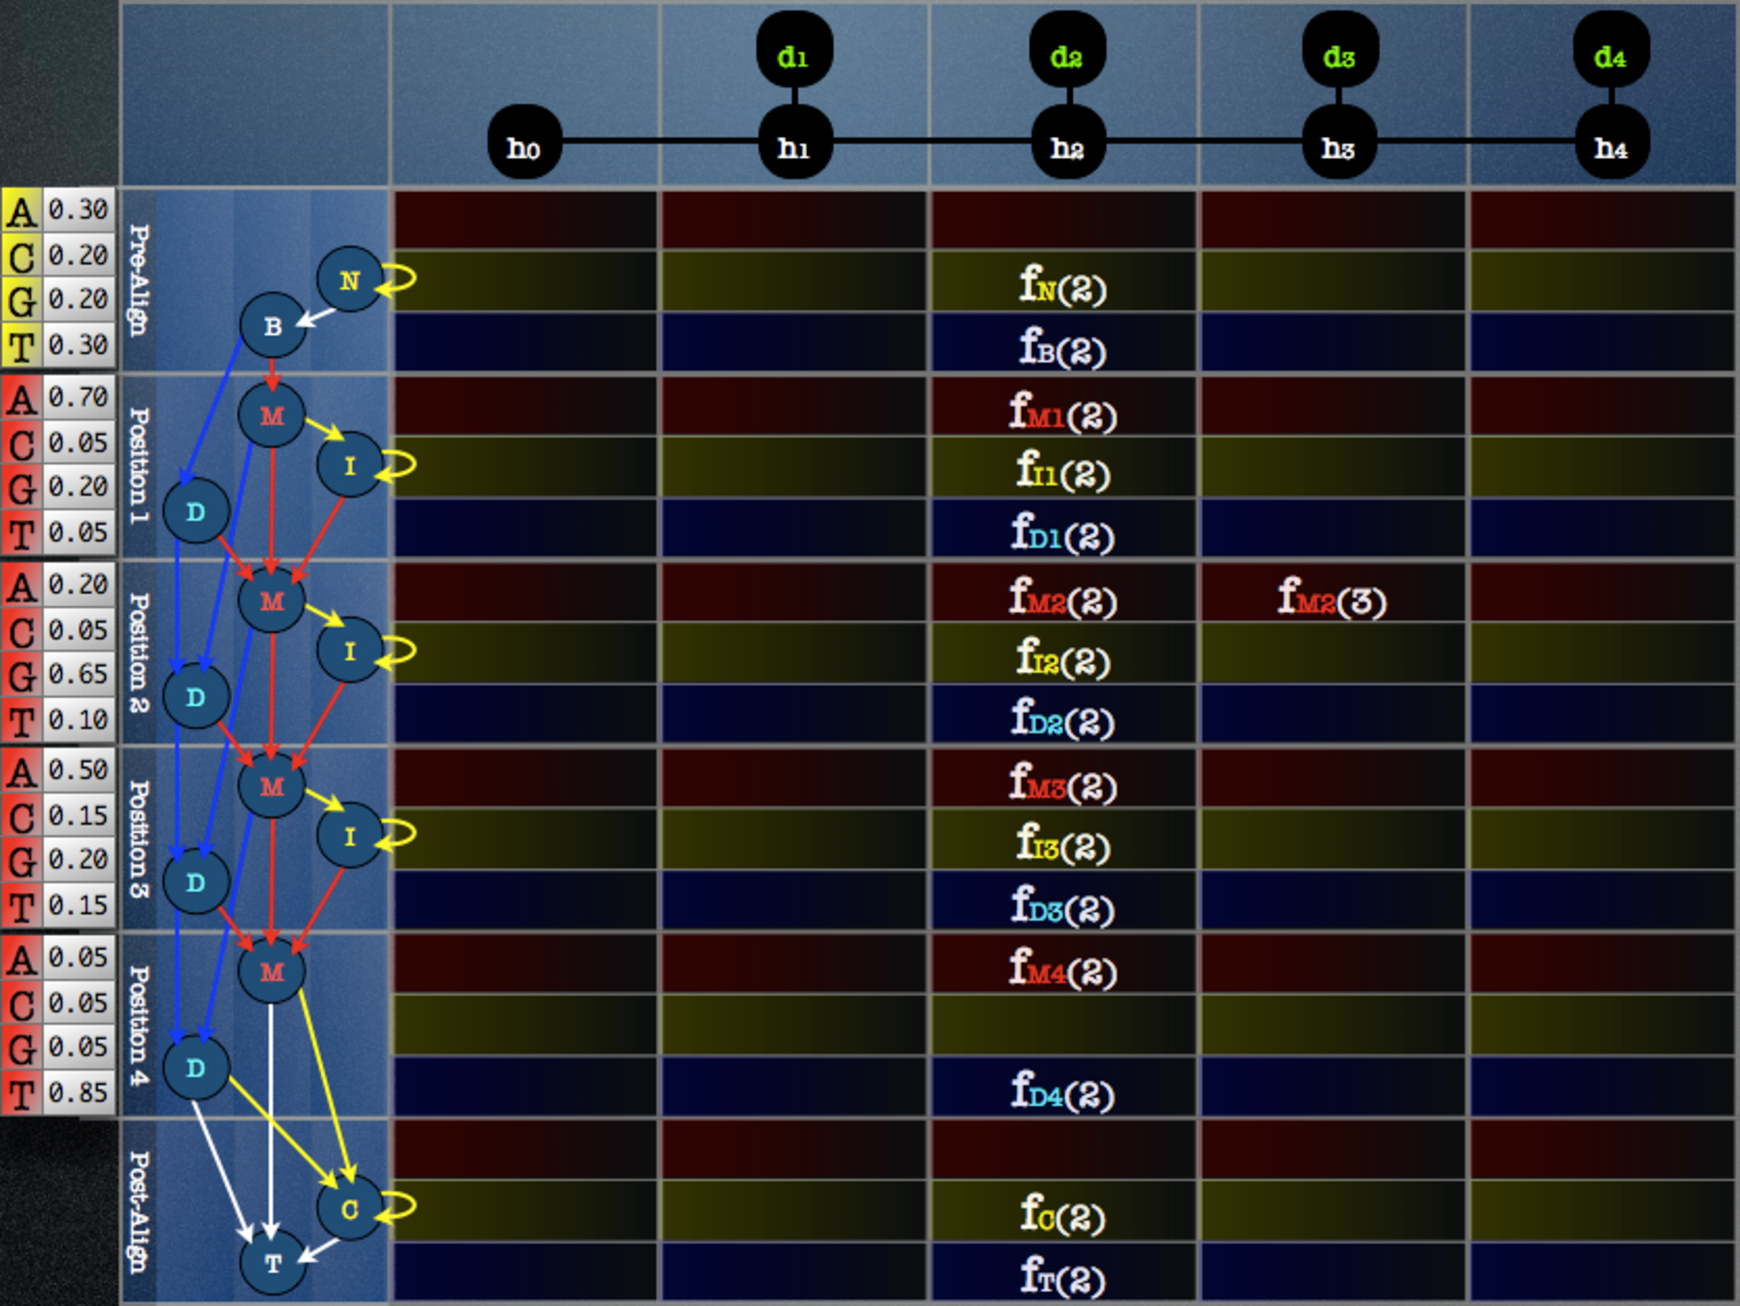
\includegraphics[scale=.35]{Plan7ForwardInTime.pdf}} \\
\subfigure[Constrained forward update]{\label{cbw_fig:Plan7ForwardByState_Match}\centering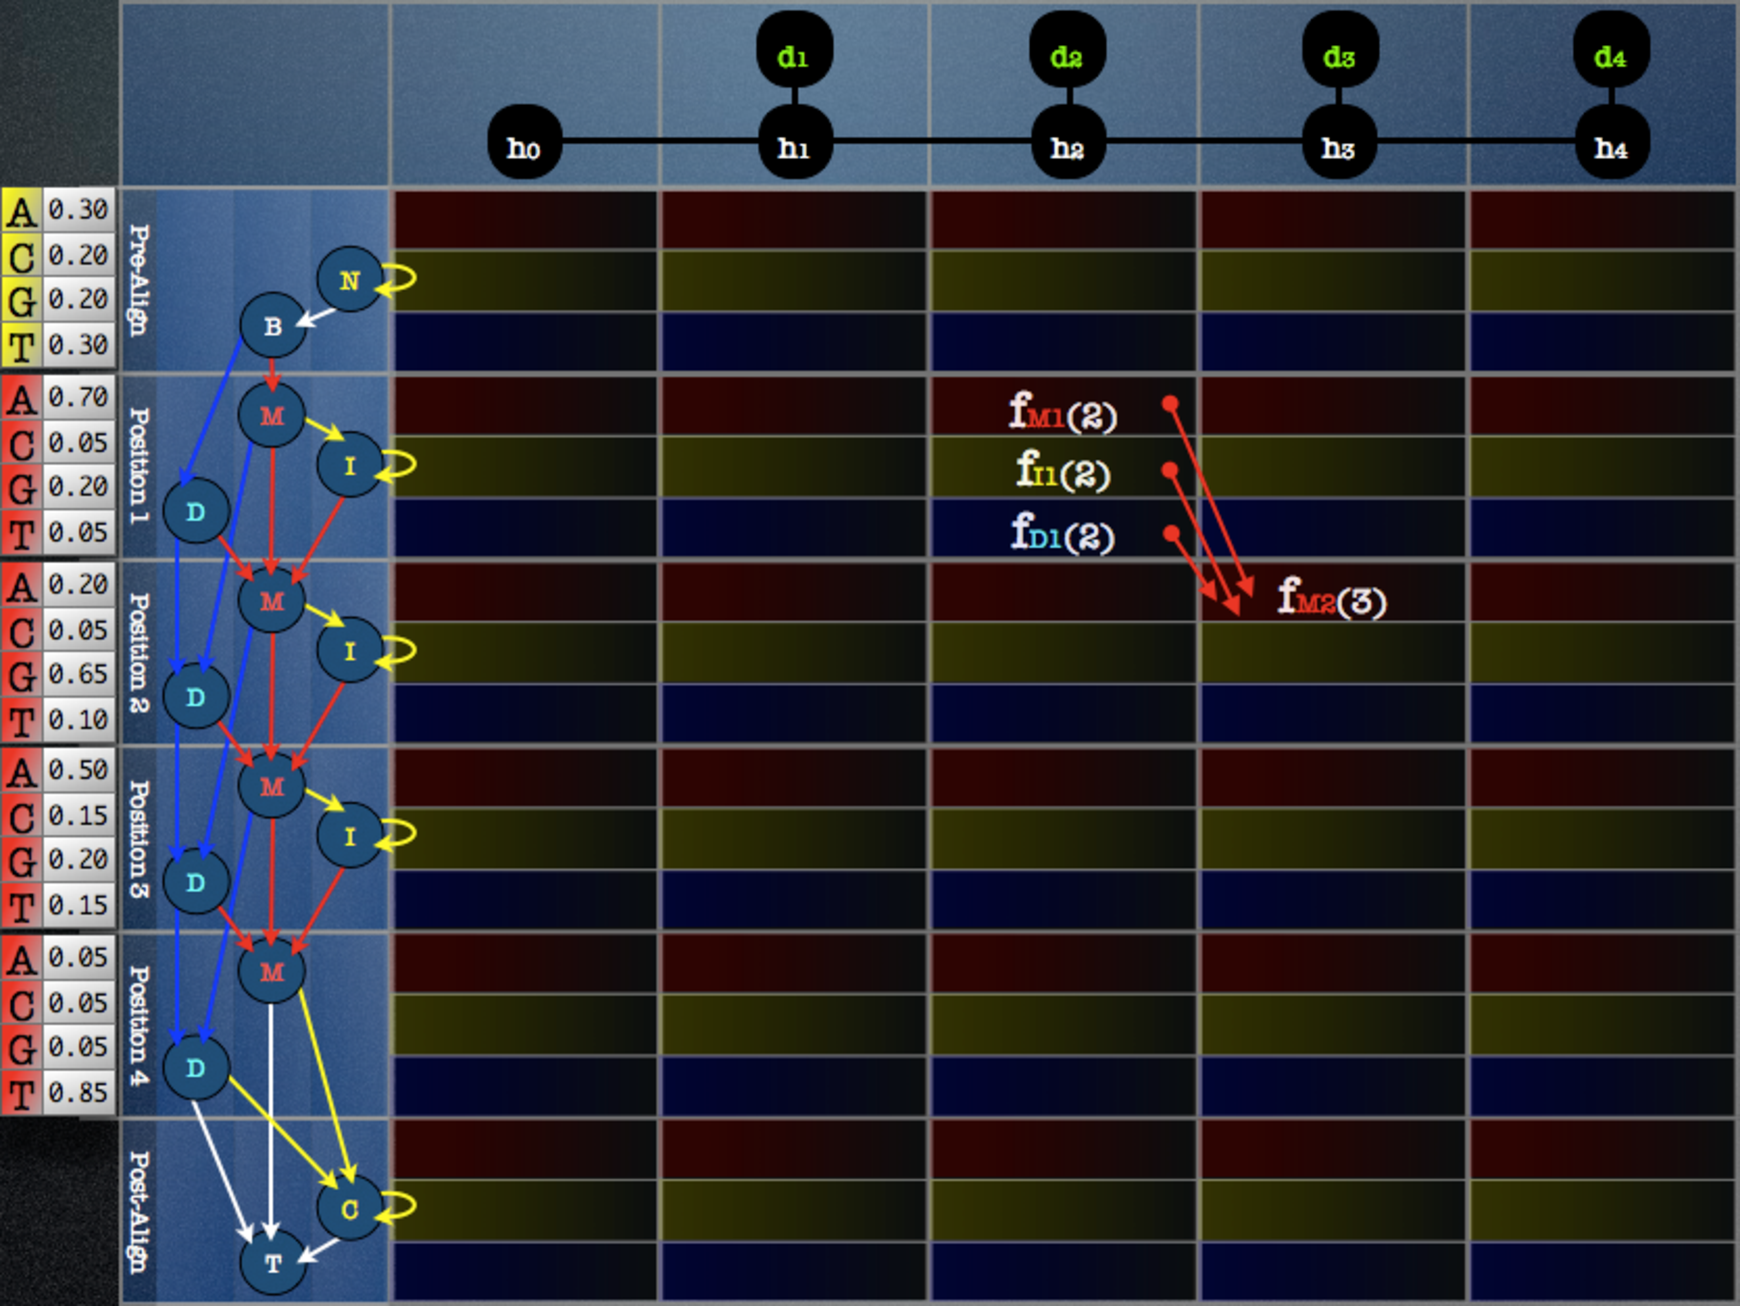
\includegraphics[scale=.35]{Plan7ForwardByState_Match.pdf}} \\
 \caption{\textbf{Forward calculation in a Profile HMM.}  The general time-oriented forward calculation (of a Match state) is shown in (a).  Since most transitions are not allowed, only the transitions denoted by arrows in (b) are relevant.  This constraint is utilized by the Conditional Baum-Welch and Conditional Quadratic Ascent algorithms to update parameters state-by-state efficiently.}
  \label{cbw_fig:Plan7ForwardInTimeandByState_Match}
\end{figure}

In some models it becomes convenient to allow for non-emitting states.  In the Profile HMM, for example, we allow for Deletion states, which are non-emitting.  Technically this is simply a convenient way to conceptualize and compute when certain transitions are geometrically-distributed: the Deletion states could be replaced by transitions between non-adjacent Match states.  By adding non-emitting states, some HMMs that do not satisfy the constraint required for CBW and CQA can be restructured to do so.

Transitions to non-emitting states are most conveniently represented as transitions that take no time (since each time is associated with an emitted datum).  When the HMM has non-emitting states, Equation~\ref{cbw_eq:forwardByStateStrict} becomes
\begin{equation}\label{cbw_eq:forwardByState}
\forward_{\Time}( \state_j )
= \sum_{i \in (j-k), \dots, j}{ \bigl( \forward_{\Time}( \state_i ) \HMMtransitionLaw( \state_j | \state_i )\bm{1}^{\not{\hbox{e}}}(\state_j) + \forward_{\Time - 1}( \state_i ) \HMMtransitionLaw( \state_j | \state_j ) \HMMemissionLaw( \datum_{\Time} | \state_j )\bm{1}^{\hbox{e}}(\state_j) \bigr) } \hbox{,}
\end{equation}
where $\bm{1}^{\hbox{e}}(\cdot)$ is the function indicating whether its argument state is emitting, and $\bm{1}^{\not{\hbox{e}}}(\cdot)$ is the function indicating whether its argument state is non-emitting.  Figure~\ref{cbw_fig:Plan7ForwardByState_Deletion} depicts the forward update for a Deletion state of the Profile HMM.

\begin{figure}[htp]
\centering
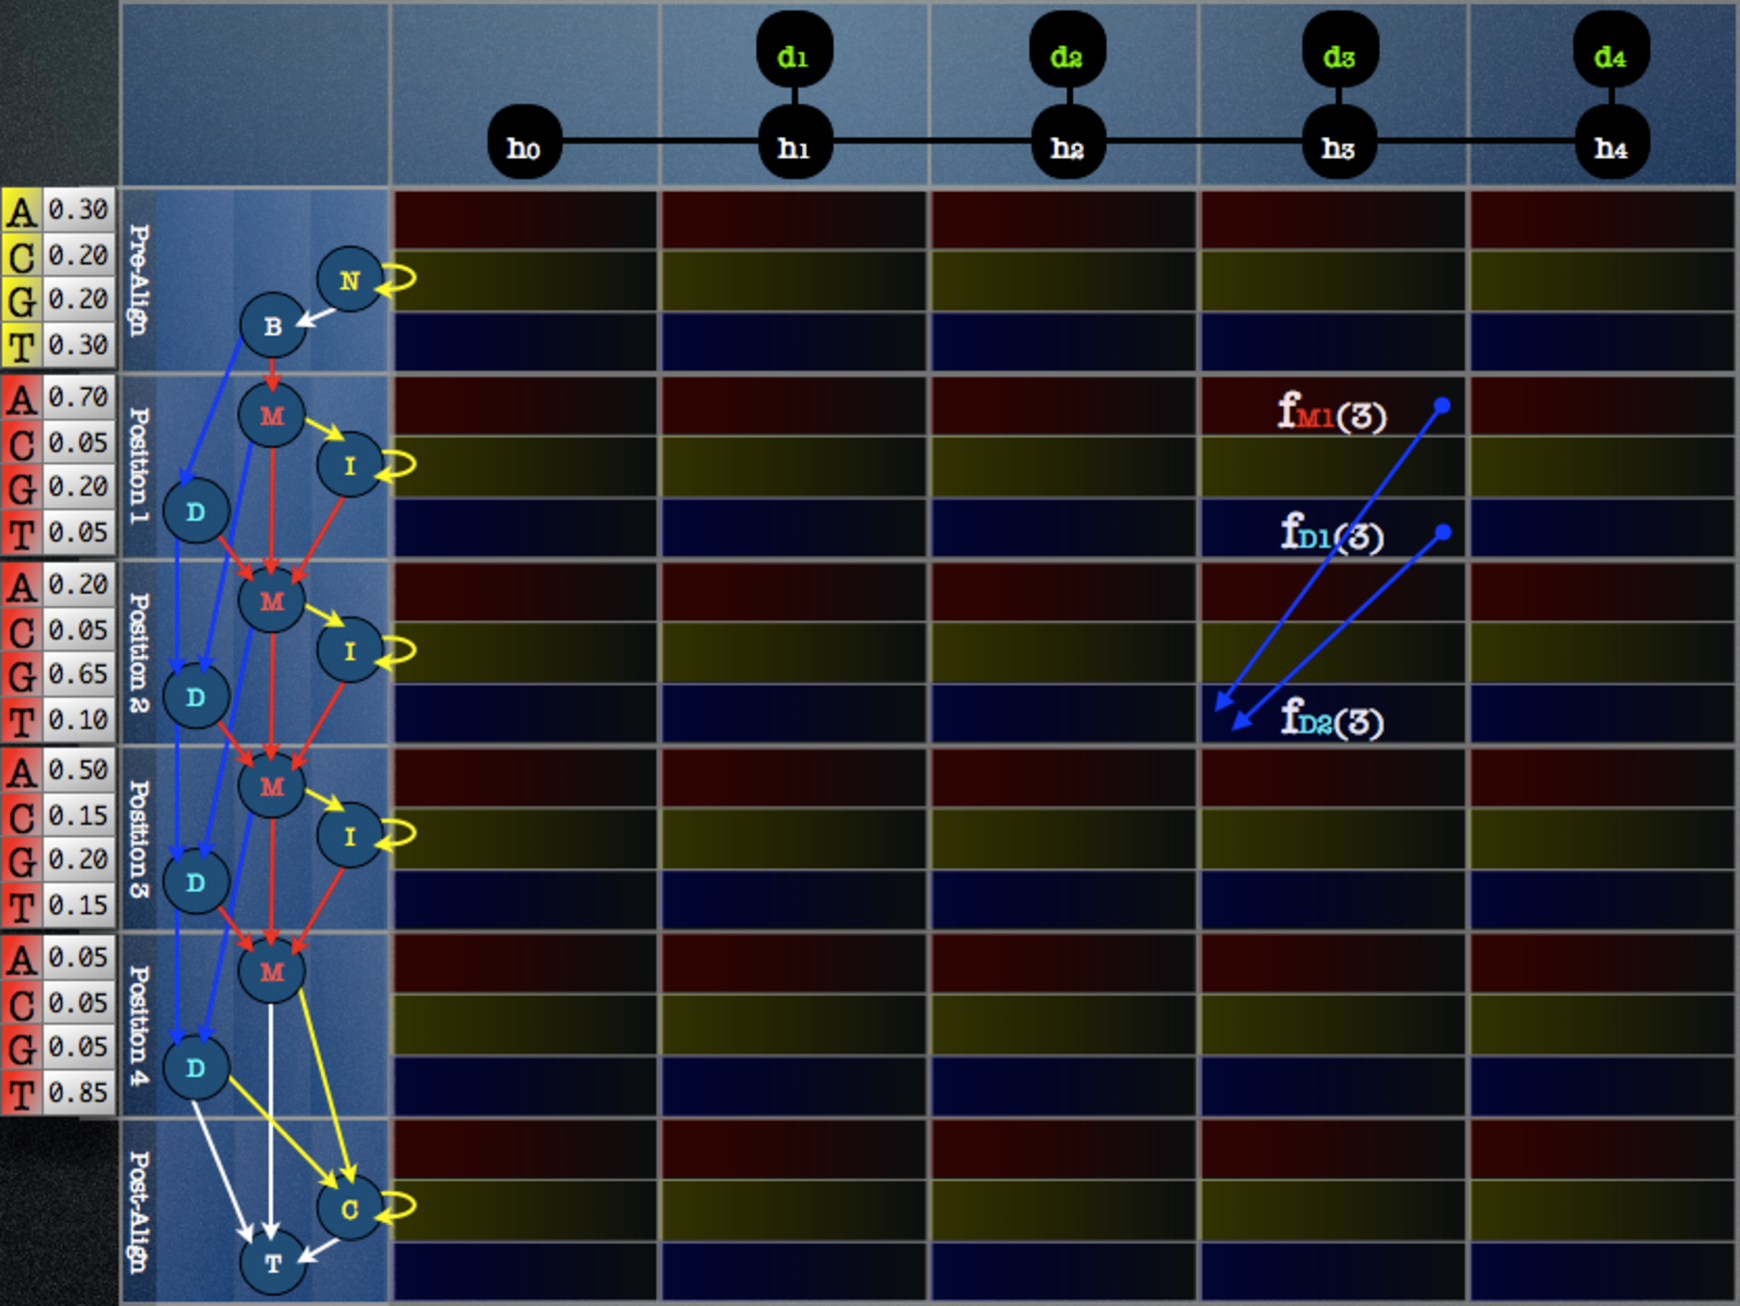
\includegraphics[scale=.35]{Plan7ForwardByState_Deletion.pdf} \\
 \caption{\textbf{Forward calculation of a non-emitting state in the Profile HMM.}  Since Deletion states in Profile HMMs are non-emitting, transitions to them are within one column.}
  \label{cbw_fig:Plan7ForwardByState_Deletion}
\end{figure}

The CBW and CQA algorithms compute the forward and backward values row-by-row (state-by-state) rather than column-by-column (time-by-time) (Figure~\ref{cbw_fig:BW_vs_CBW}).  Since the calculation of the forward values in a row depends only on the parameters affecting the states of that row, and on the forward values of the previous row, the CBW and CQA algorithms only need to recompute the forward values of the affected row.  The algorithms proceed row-by-row, updating the group of parameters associated with the states of that row.  After the update, the algorithms calculate the forward values of the affected row, then proceed to the next row.  Since each forward value needs to be calculated only once, the total computational cost of these algorithms is on the same order as that of the BW algorithm (bilinear in the number of states and the total length of all observation sequences).

\begin{figure}[htp]
\centering
\subfigure[BW update: column-by-column]{\label{cbw_fig:BW_vs_CBW_BW}\centering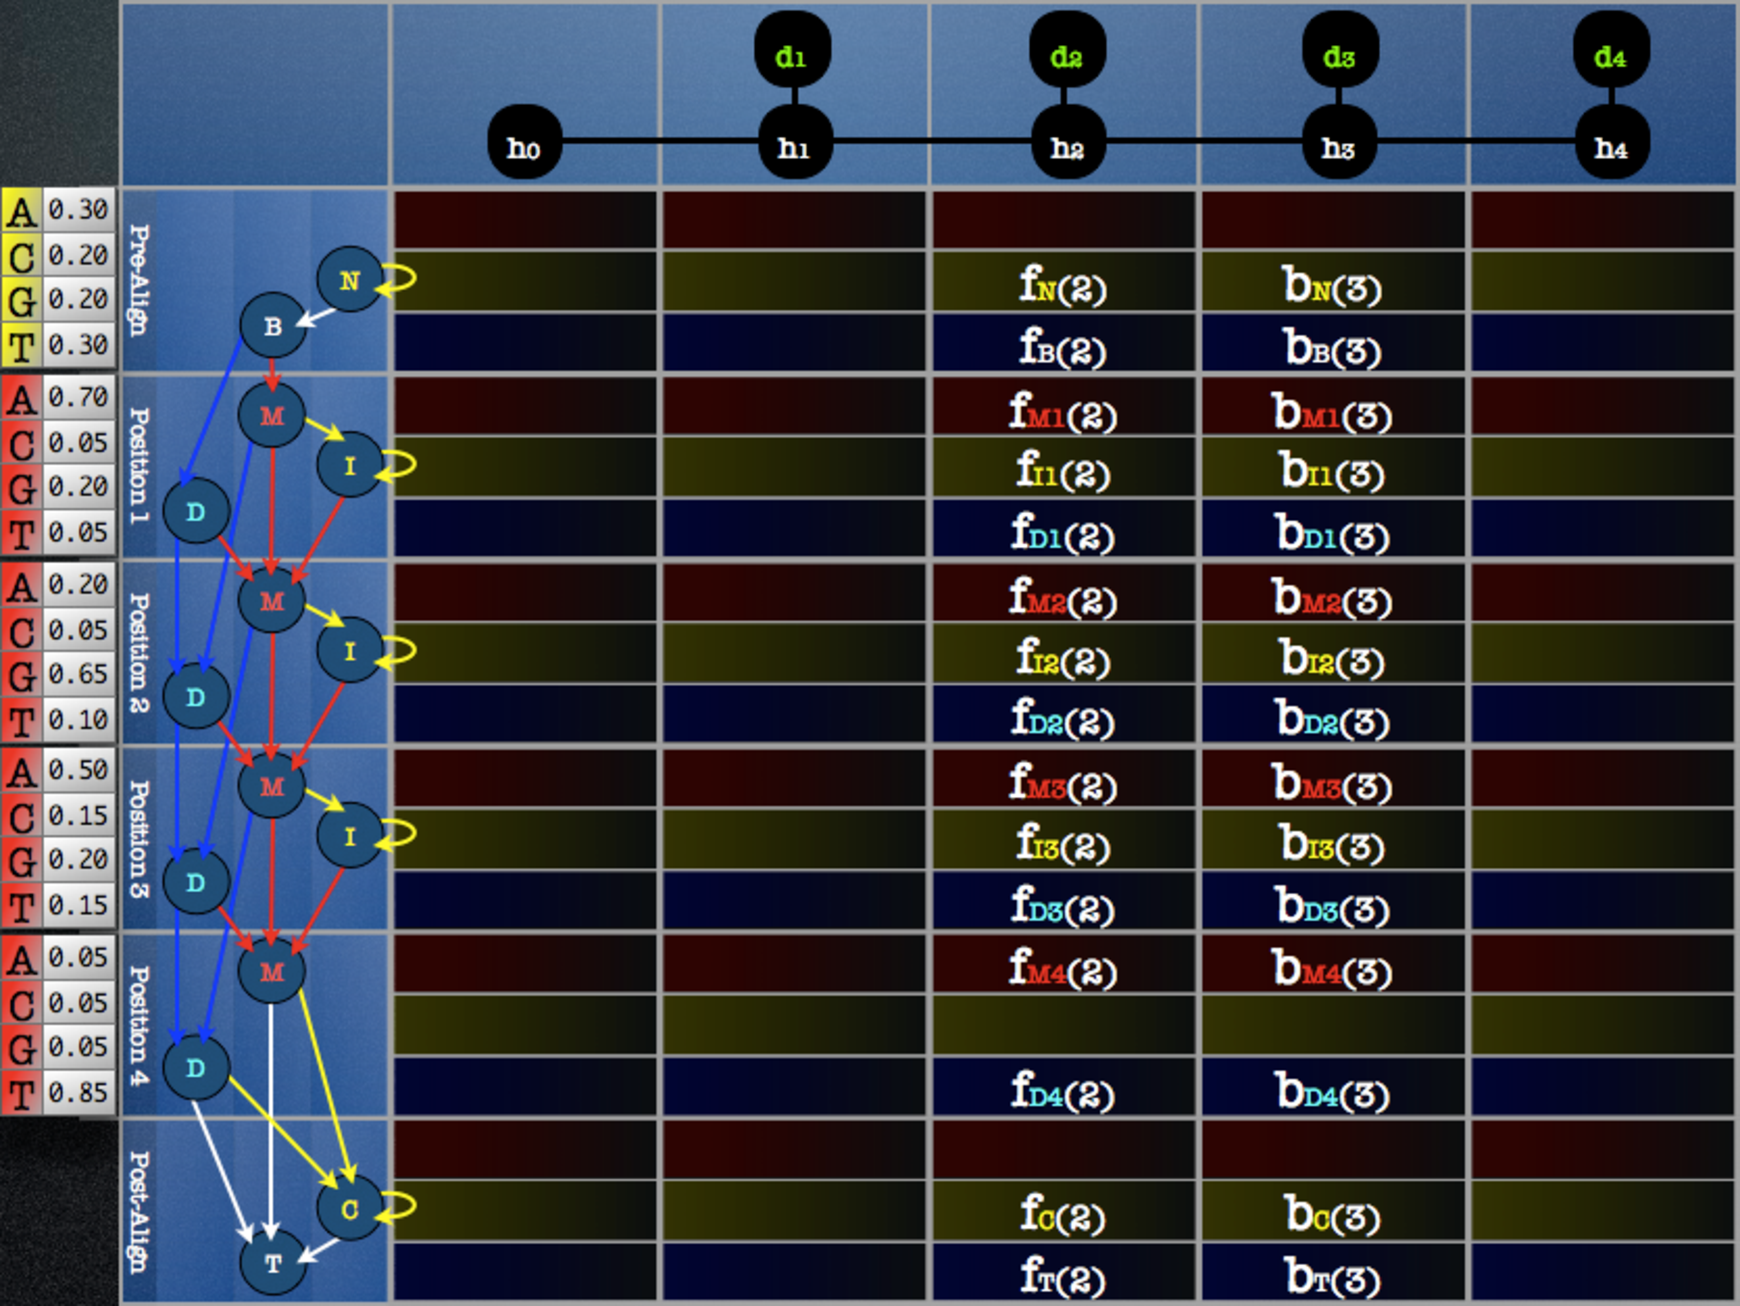
\includegraphics[scale=.35]{BW_vs_CBW_BW.pdf}} \\
\subfigure[CBW and CQA updates: row-by-row]{\label{cbw_fig:BW_vs_CBW_CBW}\centering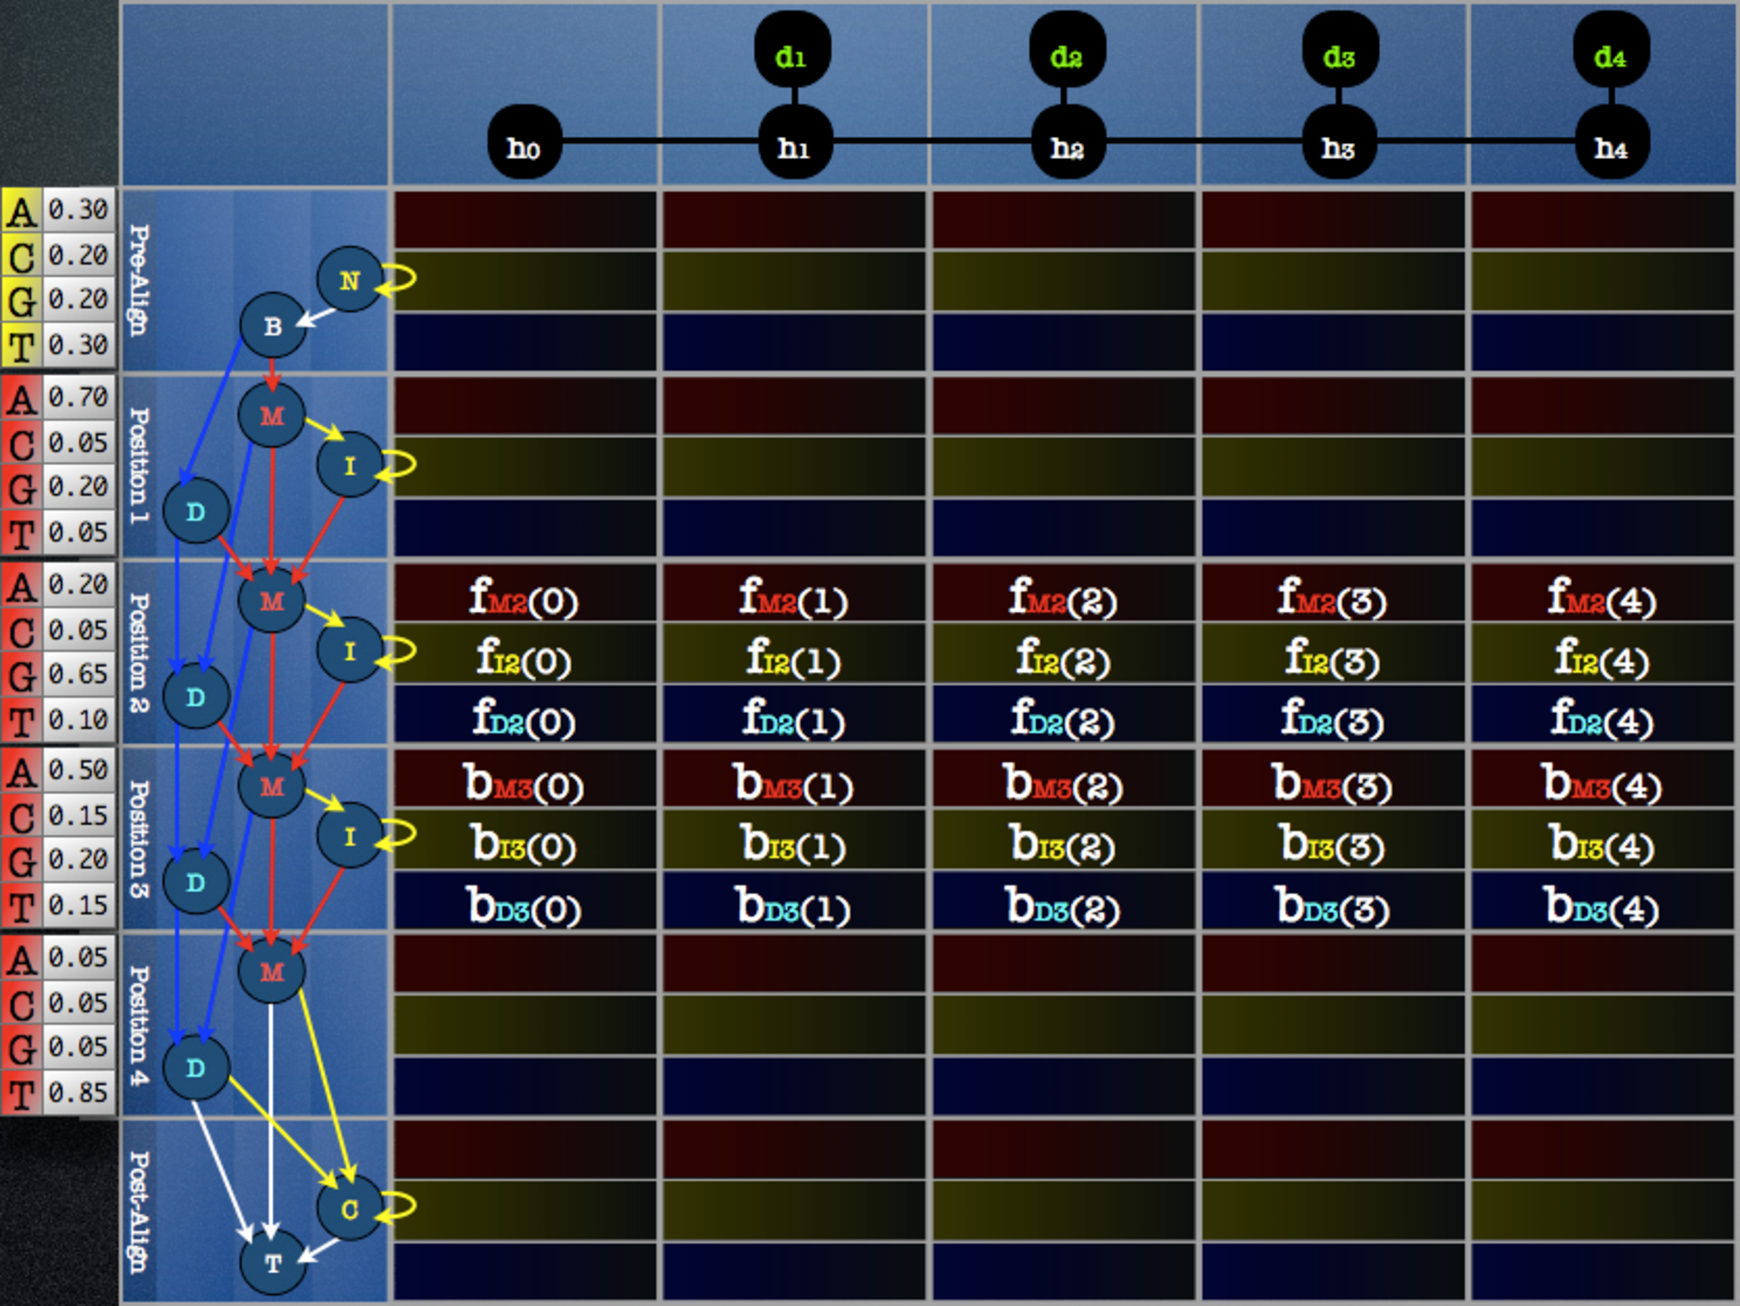
\includegraphics[scale=.35]{BW_vs_CBW_CBW.pdf}} \\
 \caption{\textbf{Baum-Welch, Conditional Baum-Welch, and Conditional Quadratic Ascent in a Profile HMM.}  The values used in the time-oriented Baum-Welch update calculation are shown in (a).  Conditional Baum-Welch and Conditional Quadratic Ascent instead calculate updates in blocks of states.  (b) shows the values used in the CBW or CQA update of the parameters affecting the three states (M, I, and D) associated with position 3.  The CBW and CQA algorithms progress in blocks of states, using the updated parameters to recalculate the forward values as they proceed.}
  \label{cbw_fig:BW_vs_CBW}
\end{figure}

We showed in \cite{edlefsen2010transposon} that the
CBW algorithm can outperform the BW algorithm across a range of
simulation conditions, as well as in the biological context of
identifying transposons in DNA sequences.  In the results section below we show that the alternative approach of directly maximizing by gradient ascent (CQA) performs at least as well as the CBW procedure and better in cases relevant HIV-1 within-host evolution studies.

\section{Quadratic Ascent}
The Baum-Welch and Conditional Baum-Welch algorithms ascend the
likelihood (or the posterior distribution of the parameters) by
maximizing a surrogate function that is guaranteed to be below the
target function.  EM algorithms such as these are useful for maximizing complicated
functions for which direct analytical or numerical maximization is
impossible or impractical.  While no analytical solution exists for
directly maximizing the parameters of Profile HMMs, the gradient of
the log-likelihood (after normalized exponential transformation) has a simple
analytical solution, suggesting direct optimization methods such as gradient
ascent.  Pierre Baldi and Yves Chauvin derived
this gradient and introduced gradient ascent procedures for Profile HMMs in their
landmark 1994 papers \citep{Baldi:1994, baldi1994smooth}.  \cite{Mamitsuka:1996, Mamitsuka:1998} introduced a closely related method that differs only in the
determination of the step size.

%% TODO: Add note to discussion about how use of priors would regularize the overfitting.

To our knowledge, apart from the original articles, these gradient
ascent methods have not been widely adopted for estimating parameters
of Profile HMMs, despite the oft-noted tendency of the dominant
Baum-Welch approach to prematurely converge.  Our implementation of
the Baldi-Chauvin methods reveals a possible explanation for the
relative obscurity of gradient ascent for PHMMs: the parameters
(temperature and learning rate) have optima that depend sensitively on
the training sequences, and even with optimized parameters the methods
perform poorly in comparison to the Baum-Welch approach.  Since the
appropriate step length is not analytically available, methods must be
employed for exploring the step length.  Unfortunately, such methods
typically require repeatedly employing a costly recalculation of the
target function (in this case, the forward algorithm to determine the
likelihood).

Our original (unpublished) efforts to estimate parameters for PHMMs
led us serendipitously to the approach that we introduce here as
Quadratic Ascent: inspired by the Backprop algorithm
\citep{Rumelhart:1986}, and unaware of the applicability of existing
methods for HMMs, we devised a conditional maximization approach based
on isolating subsets of the parameters, transforming them to a
normalized exponential representation to eliminate the boundary
constraints, and then sampling perturbations to determine a gradient.
This method determines locally optimal step sizes by fitting a
quadratic function (a parabola) to the log-likelihood (as a function
of the step size) and updates the parameters by climbing the gradient
to the estimated peak.  The Quadratic Ascent method is essentially
identical to this original method, except that we replace the gradient
estimation step with the Baldi-Chauvin analytical gradient.

As in \cite{Baldi:1994}, we transform the variables for each
parameter distribution $\ParametersSubset$ (supported on a simplex) to unconstrained values
$\boltzmannTransformedParameter \in \BoltzmannTransformedParameters$ such that for each
$\parametersSubsetParameter \in \ParametersSubset$,
$\parametersSubsetParameter =
\frac{\exp(\boltzmannTransformTemperature
  \boltzmannTransformedParameter)}{\sum_{\boltzmannTransformedParameter'
    \in \BoltzmannTransformedParameters}{\exp(\boltzmannTransformTemperature \boltzmannTransformedParameter')}}$.
This transformation uniquely defines parameters $\boltzmannTransformedParameter \in
\BoltzmannTransformedParameters$ for any fixed
$\parametersSubsetParameter \in \ParametersSubset$, given temperature
$\boltzmannTransformTemperature$.  We find that a temperature value of
$\boltzmannTransformTemperature = 1$ suffices and set it thus for the
results presented below.

Baldi and Chauvin showed that the partial derivative of the
log-likelihood with respect to transformed parameter
$\boltzmannTransformedParameter$ (corresponding to untransformed
parameter $\parameter$) is 
\begin{equation*}
\begin{split}
\frac{\partial \log \Prob ( \Sequences \big| \Parameters )}{\partial \boltzmannTransformedParameter}
 &= \boltzmannTransformTemperature \sum_{\sequenceIndex}{ \frac{
     \ExpectedCounts_{\sequenceIndex}( \parameter ) -
     \bwParameterValue \TotalExpectedCounts_{\sequenceIndex} \left(
       \multinomial( \parameter ) \right) } {
     \Prob ( \vec{\datum}_{\sequenceIndex} \big| \Parameters ) } } \hbox{,}
\end{split}
\end{equation*}
where  $\bwParameterValue$ is the Baum-Welch
update for parameter $\parameter$, $\ExpectedCounts_{\sequenceIndex}( \parameter )$ is the expected number of uses
of parameter $\parameter$ while generating the observed sequence at
index $\sequenceIndex$ (using the current parameters, $\Parameters$) and
$\TotalExpectedCounts_{\sequenceIndex} \left( \multinomial( \parameter ) \right)$ is
the sum of $\ExpectedCounts_{\sequenceIndex} ( \otherParameter )$ over all parameters
$\otherParameter$ of the multinomial distribution
$\multinomial( \parameter )$ of which
$\parameter$ is a component.

Given a known step size $\qaStepSize$, each set of parameters is
updated in the transformed space by adding $\qaStepSize \nabla \log
\Prob ( \Sequences \big| \Parameters )$ to the transformed parameters
$\BoltzmannTransformedParameters$.  The Baldi-Chauvin method, which
also includes an ``online'' variant of this procedure to compute
per-sequence parameter updates, does not specifically address the
choice of $\qaStepSize$ \citep{baldi1994smooth}.  Our contribution is two-fold: first, we
introduce a simple quadratic line search approach for dynamically
computing the step size $\qaStepSize$ for each update, and second, by
employing the same ``rotated'' approach as is used in Conditional
Baum-Welch, our Conditional Quadratic Ascent procedure isolates and
updates subsets of parameters at a time (we do this for all sequences
simultaneously, though an ``online'' variant would be a
straightforward extension).  Without employing dynamically computed step sizes,
we find that the original fixed-step-size Baldi-Chauvin method behaves poorly in
comparison to all other methods presented here (data not shown).

Our dynamic computation of step sizes depends on repeatedly
recomputing the target function (the likelihood) at various step size
proposals.  The efficiency of this recomputation is important because
it is repeatedly applied for each step size determination.  In
general, the time to compute the likelihood is on the same order as a
complete Baum-Welch update (or a whole sweep of Conditional Baum-Welch
updates).  Without careful optimization, the time cost would be
prohibitive for most real-world applications, since each Quadratic
Ascent update would require many times more computation than a
Baum-Welch update.  This is especially true for Conditional Quadratic
Ascent, which computes a separate step size for each update of each
position-specific subset of the parameters.  While technically the
time complexity of Quadratic Ascent remains the same as that of
Baum-Welch so long as the number of recalculations per step size
determination is bounded (eg by setting a hard limit), the time
required for Quadratic Ascent would be prohibitively worse than that
of Baum-Welch.

Fortunately, we have discovered that for each parameter subset update
step of the Conditional Quadratic Ascent algorithm, the recomputation
of the likelihood can be performed in time proportional to the number
of sequences rather than to their total length (as would be required in a
naive implementation).  This is accomplished by representing the
probability of each individual sequence as a linear function of the
parameter subset.  So long as the parameter subset includes only
single-use parameters (ie. any but Insertion state
self-transitions), this linear function can be applied in constant
time per sequence to recompute its sequence probability as a function
of changed parameters.

In the Results section below we present results from simulation
experiments in which the transition parameters are also constrained to be
equal at all positions.  With this constraint, the only
position-specific parameters are the Match state emission parameters.
Our present implementation employs QA only for the Match emission
parameters (which are single-use), and alternates these updates with
Baum-Welch updates applied to the parameters that are not
position-specific.  It is possible to apply the QA algorithm to
parameters that are multi-use (such as Insertion self-transitions), but
since the likelihood must be expensively recomputed with each step in
the effort to isolate and ascend the local quadratic, it is slow compared to Baum-Welch.

The results demonstrate that the Conditional Quadratic Ascent method,
even as applied only to the Match emission parameters, achieves higher
and more robust maxima than Conditional Baum-Welch.

\section{Results}
\subsection{Simulation Study}
We now provide results from a simulation study in which we compared
the Conditional Baum-Welch, (Unconditional) Baum-Welch, Conditional
Quadratic Ascent, and Unconditional Quadratic Ascent algorithms across
a series of data sets randomly generated from Profile HMMs.  We split
each set of generated sequences into a training set and a test set,
and then assessed how well each algorithm performed using the
probability of the test set under a Profile HMM with parameters
estimated using the training set.  The ``true'' profiles were designed
to represent a conservation level of $0.5$ and $0.75$.  For
example a true profile with conservation level $0.5$ assigns fifty
percent probability to one (randomly determined) residue at each
position, and assigns each of the remaining residues an equal share of
the remaining probability.  Transition parameters were set such that
the expected number of insertions per generated sequence was $8$ and the
expected length of each insertion was 1.25\% of the profile length,
and likewise for deletions.

We evaluated two scenarios: for both DNA and AA sequence families we evaluated a scenario in which 100 sequences are available, and the profile length is 100.  We found that for DNA, under this scenario all four evaluated methods performed well (and were indistinguishable) at a conservation level of $0.75$, and all four methods overtrained and performed poorly on the test set at conservation level $0.5$ (data not shown).  However for AA sequences under this scenario we found that at both conservation levels, CQA and UQA outperformed CBW and UBW.  In the second scenario (evaluated only for DNA sequences families), we more closely approximated the scenario of within-host HIV-1 evolution (see below). We evaluated profiles of length 1000, using only 20 sequences for parameter estimation, with conservation rates $0.75$ and $0.90$.  In all cases we used 100 sequences for the test set.

\begin{figure}[htp]
\centering
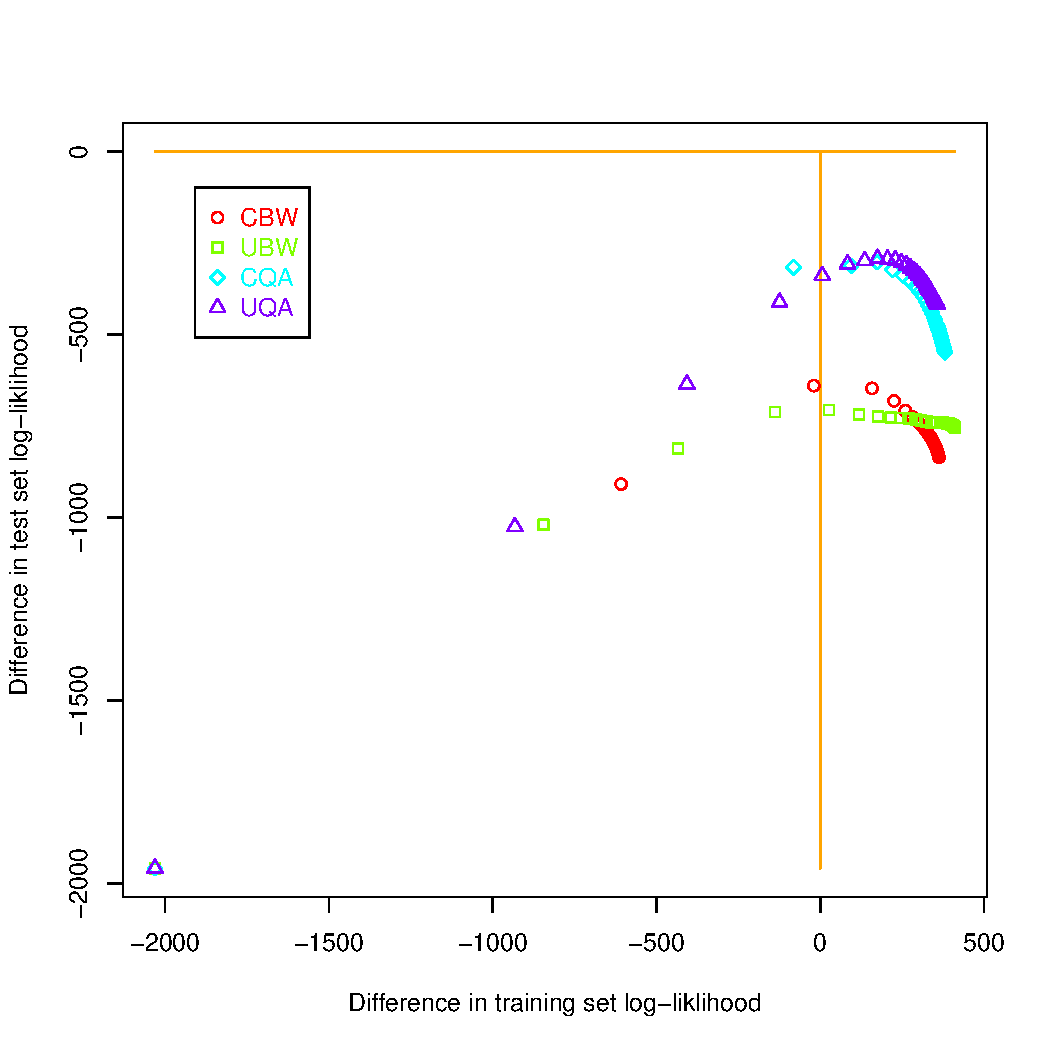
\includegraphics[scale=.85]{AA_priorstart_results_50.pdf}
\caption{\textbf{AA Simulation Results for Concentration Rate 0.50.}  AA results for the scenario with 100 sequences drawn from a profile of length 100 for a conservation rate of $0.50$ are shown, color coded by method.  The points plot the iterations of the algorithm from 0 to convergence, from left to right.  The X axis shows the difference in the $\log_{10}$ likelihood of the training set data, and the Y axis shows the difference in the test set data, with differences taken to the true model from which the data were drawn.  As expected there is some degree of overfitting on the training data, especially at later iterations. The Quadratic Ascent methods perform well.  These plots show averages over the four starting profiles drawn from the concentrated prior; results for the ``even'' start are comparable, and results for the ``uniform'' start are consistent but somewhat poorer (data not shown).}
\label{fig:AA_priorstart_results_50}
\end{figure}

\begin{figure}[htp]
\centering
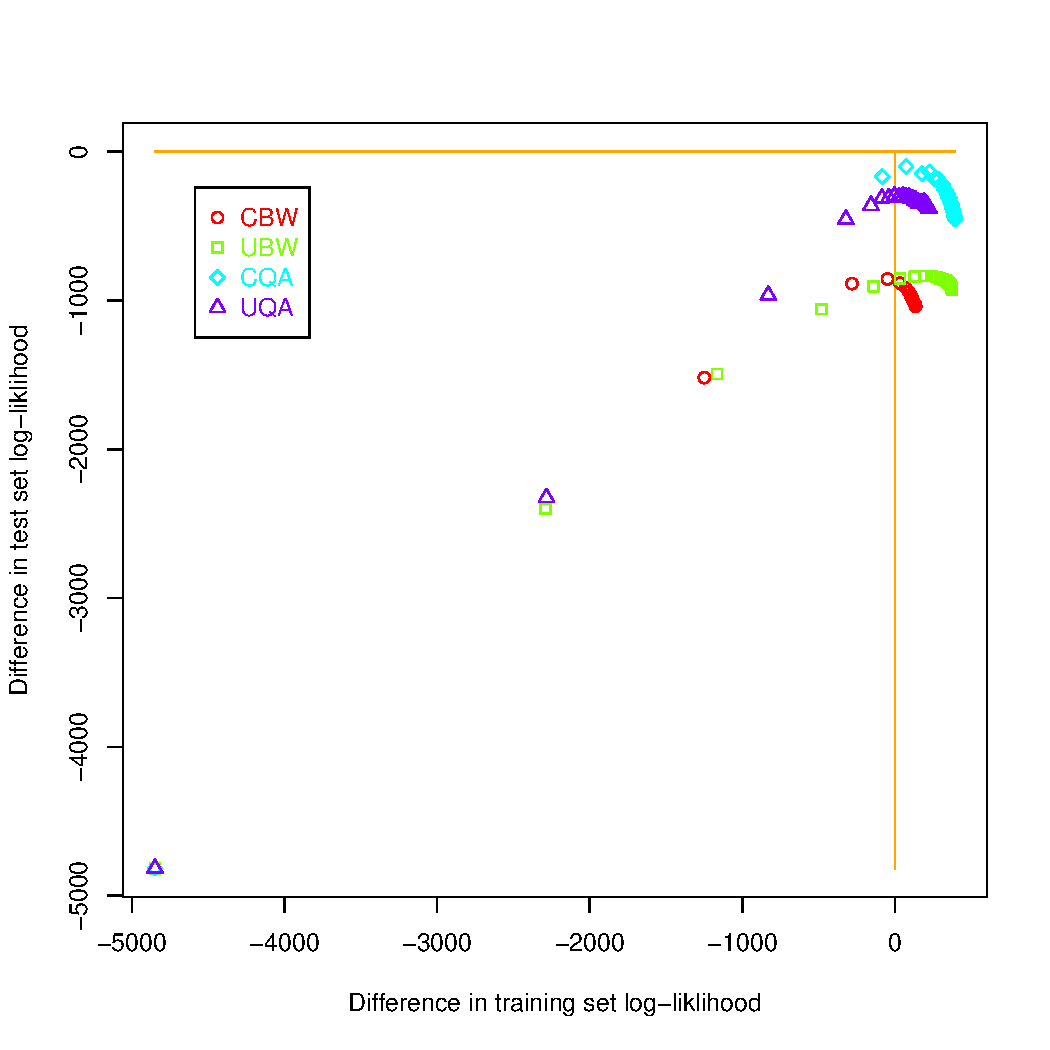
\includegraphics[scale=.85]{AA_priorstart_results_75.pdf}
\caption{\textbf{AA Simulation Results for Concentration Rate 0.75.}  AA results for the scenario with 100 sequences drawn from a profile of length 100 for a conservation rate of $0.75$ are shown, color coded by method.  The points plot the iterations of the algorithm from 0 to convergence, from left to right.  The X axis shows the difference in the $\log_{10}$ likelihood of the training set data, and the Y axis shows the difference in the test set data, with differences taken to the true model from which the data were drawn.  As expected there is some degree of overfitting on the training data, especially at later iterations. The Quadratic Ascent methods perform well.  These plots show averages over the four starting profiles drawn from the concentrated prior; results for the ``even'' start are comparable, and results for the ``uniform'' start are consistent but somewhat poorer (data not shown).}
\label{fig:AA_priorstart_results_75}
\end{figure}


For each of the true
profiles we created nine ``starting'' profiles: one with ``even''
Match emission probabilities (eg. each residue having equal
probability), four with Match emission probabilities chosen uniformly
at random, and four with Match emission probabilities drawn from a
symmetric Dirichlet with concentration parameter 100.  We trained each
true profile nine times per algorithm, once from each of the nine
starting profiles.  The algorithms were assessed by the probability
they assigned to the training set and by the probability they assigned
to the test set.

Experience has taught us that the algorithms are not very sensitive to
the starting values of the transition parameters so long as they are
initially set to strongly favor Matches over gaps.  Thus we drew the
transition values of starting profiles from constrained uniform
distributions, with the initial transition probabilities from Match
states set with Match$\rightarrow$Deletion and Match$\rightarrow$Insertion transition probabilities each uniform over (0, 0.05).  Each gap extension
probability was drawn from a uniform distribution over (0, 0.5).

While it would be possible to use priors for regularization during parameter estimation \citep[treated as pseudocounts; see][]{edlefsen2010transposon}, instead a minimum value of 1E-5 was enforced for
all parameter values being trained, to prevent the algorithms from
getting trapped with zero-valued parameters.  The algorithms were run until convergence, with convergence defined as the average euclidean distance of all free parameters being less than 1E-5.

Code for running the simulations is available at \citep[url: ][]{ProfillicSimulation} using the ``Profillic'' implementations of Unconditional Baum-Welch (UBW), Conditional Baum-Welch (CBW), Unconditional Quadratic Ascent (UQA), and Conditional Quadratic Ascent (CQA) \citep[url: ][]{Profillic}.

Figures~\ref{fig:AA_priorstart_results_50}~and~\ref{fig:AA_priorstart_results_75} plot the progress of the algorithms when applied to AA sequence families for the first scenario, in terms of the difference at each iteration in training set log-likelihood (on the X axis) versus the difference in the test set log-likelihood (on the Y axis), with differences taken between the estimated model and the true model that generated the data.  Figures~\ref{fig:DNA_priorstart_results_75}~and~\ref{fig:DNA_priorstart_results_90} show the analogous results for DNA sequence families under the second scenario.  The points in the lower left coincide because all four algorithms begin with the same random starting PHMM; thereafter the points trace the algorithm's optimization path (left to right).  The corresponding performance versus the true profile increases as the algorithms progress, however in every case there is evidence of some degree of overfitting, as indicated by the drop in the curves to the right of the zero line.  Starting from models with position emission probabilities more concentrated around the even distribution turns out to be an important advance, as shown by contrast to Figures~\ref{fig:DNA_uniformstart_results_75}~and~\ref{fig:DNA_uniformstart_results_90}, which start with draws from a dirichlet(1,1,1,1) distribution.

\begin{figure}[htp]
\centering
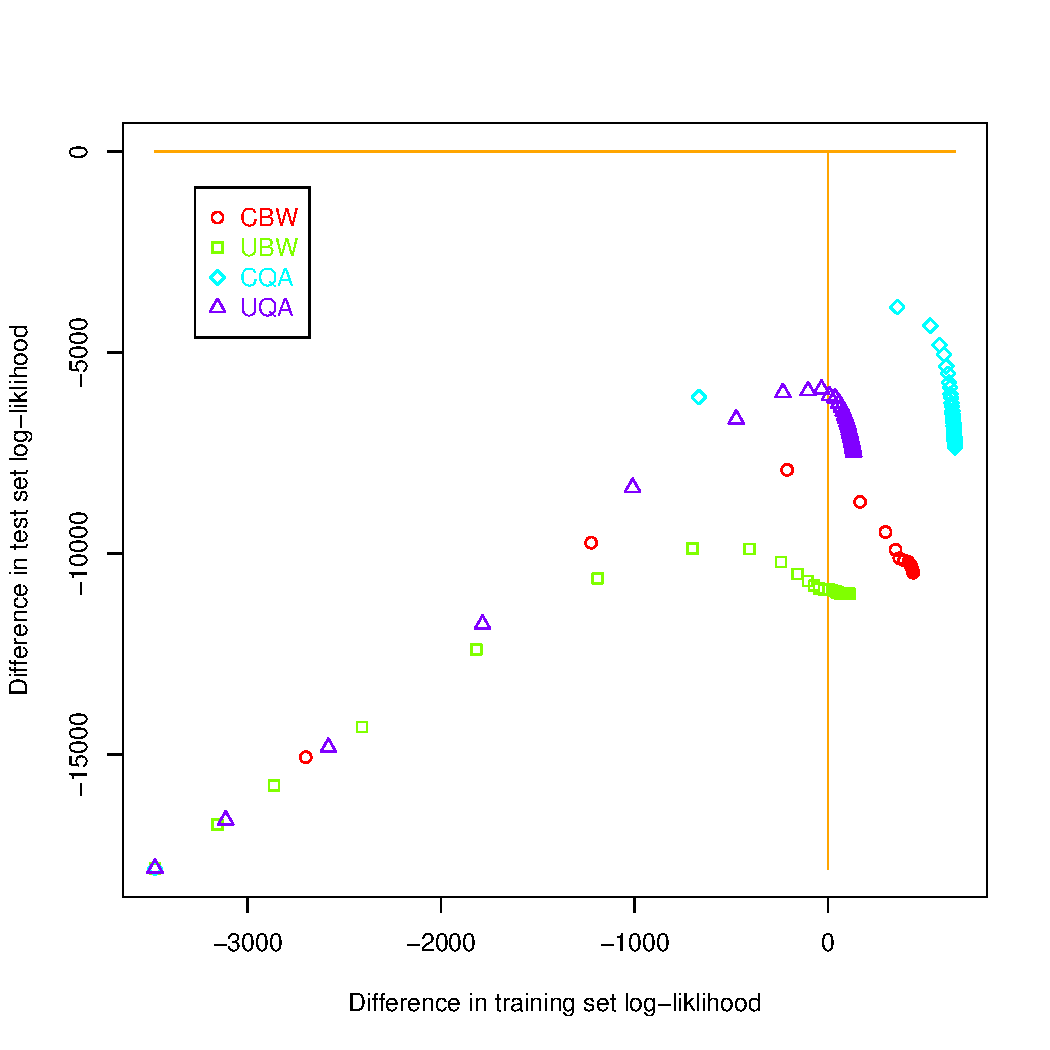
\includegraphics[scale=.85]{DNA_priorstart_results_75.pdf}
\caption{\textbf{DNA Simulation Results for Concentration Rate 0.75, starting from concentrated prior.}  DNA results for the scenario with 20 sequences drawn from a profile of length 1000 for a conservation rate of $0.75$ are shown, color coded by method.  The points plot the iterations of the algorithm from 0 to convergence, from left to right.  The X axis shows the difference in the $\log_{10}$ likelihood of the training set data, and the Y axis shows the difference in the test set data, with differences taken to the true model from which the data were drawn.  As expected there is some degree of overfitting on the training data, especially at later iterations. The Quadratic Ascent methods perform relatively well.}
\label{fig:DNA_priorstart_results_75}
\end{figure}

\begin{figure}[htp]
\centering
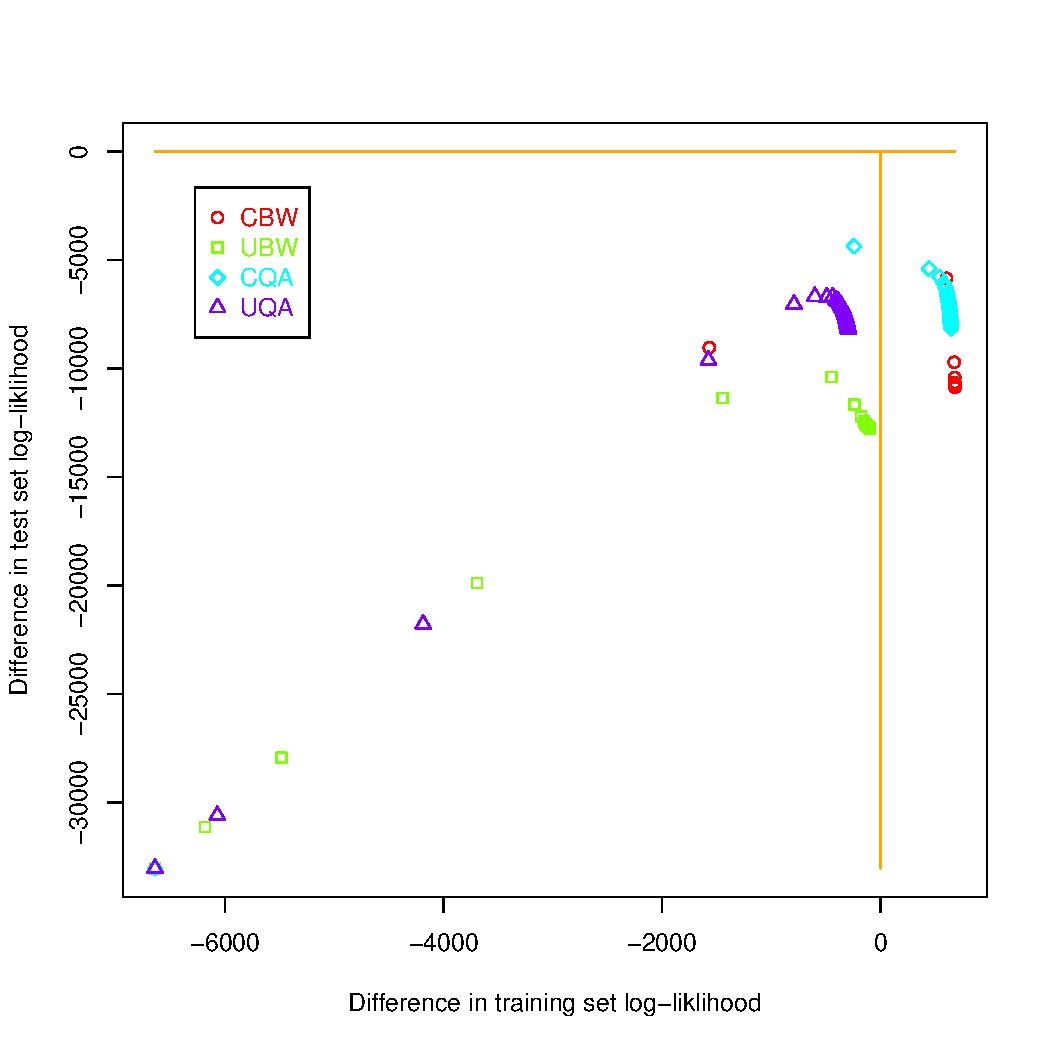
\includegraphics[scale=.85]{DNA_priorstart_results_90.pdf}
\caption{\textbf{DNA Simulation Results for Concentration Rate 0.90, starting from concentrated prior.}  DNA results for the scenario with 20 sequences drawn from a profile of length 1000 for a conservation rate of $0.90$ are shown, color coded by method.  The points plot the iterations of the algorithm from 0 to convergence, from left to right.  The X axis shows the difference in the $\log_{10}$ likelihood of the training set data, and the Y axis shows the difference in the test set data, with differences taken to the true model from which the data were drawn.  As expected there is some degree of overfitting on the training data, especially at later iterations. The Quadratic Ascent methods perform relatively well, although the inflection point of the CBW and UBW traces are obscured between iterations.}.
\label{fig:DNA_priorstart_results_90}
\end{figure}


\begin{figure}[htp]
\centering
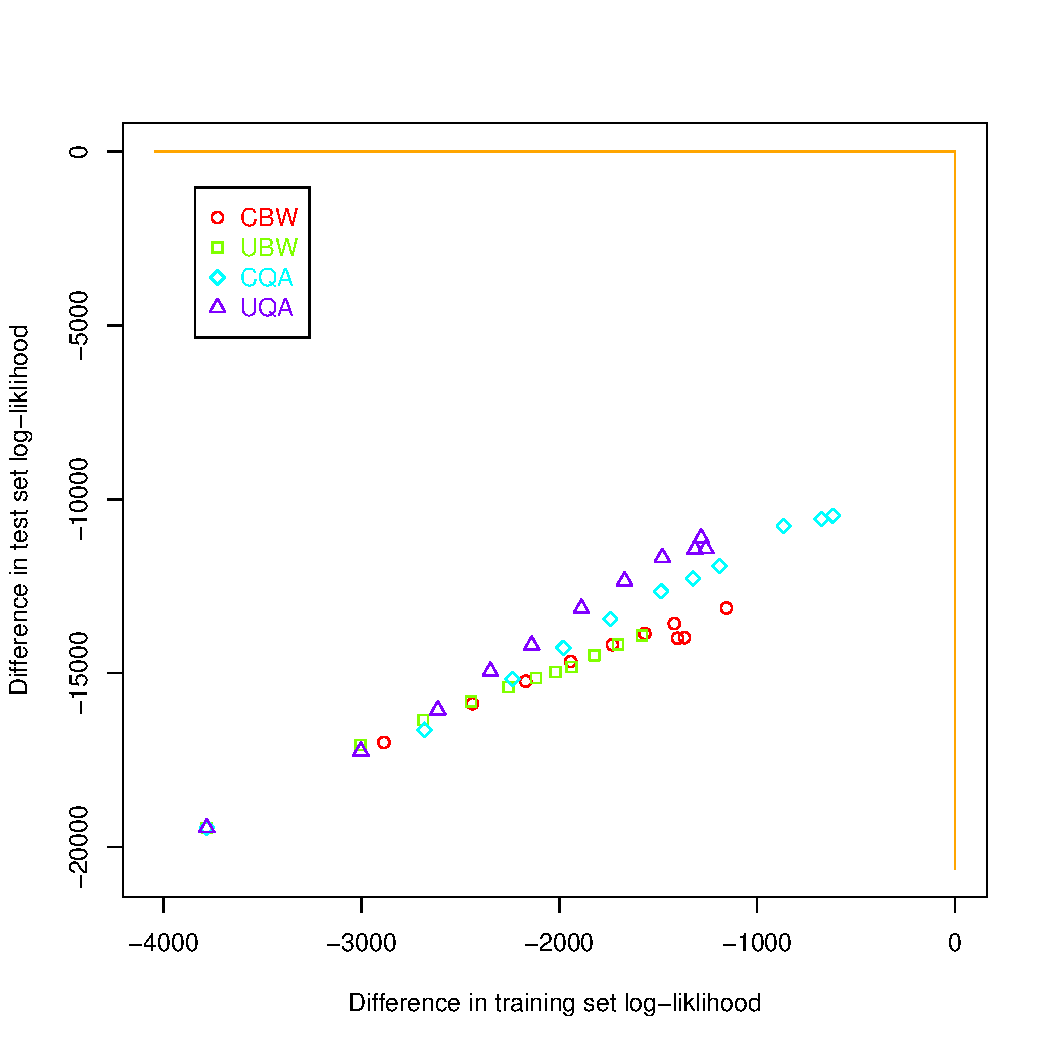
\includegraphics[scale=.85]{DNA_uniformstart_results_75.pdf}
\caption{\textbf{DNA Simulation Results for Concentration Rate 0.75, starting from uniform positions.}  DNA results for the scenario with 20 sequences drawn from a profile of length 1000 for a conservation rate of $0.75$ are shown, color coded by method.  The points plot the iterations of the algorithm from 0 to convergence, from left to right.  The X axis shows the difference in the $\log_{10}$ likelihood of the training set data, and the Y axis shows the difference in the test set data, with differences taken to the true model from which the data were drawn.  Starting from uniform positions appears to trap all of the algorithms in local optima.}
\label{fig:DNA_uniformstart_results_75}
\end{figure}

\begin{figure}[htp]
\centering
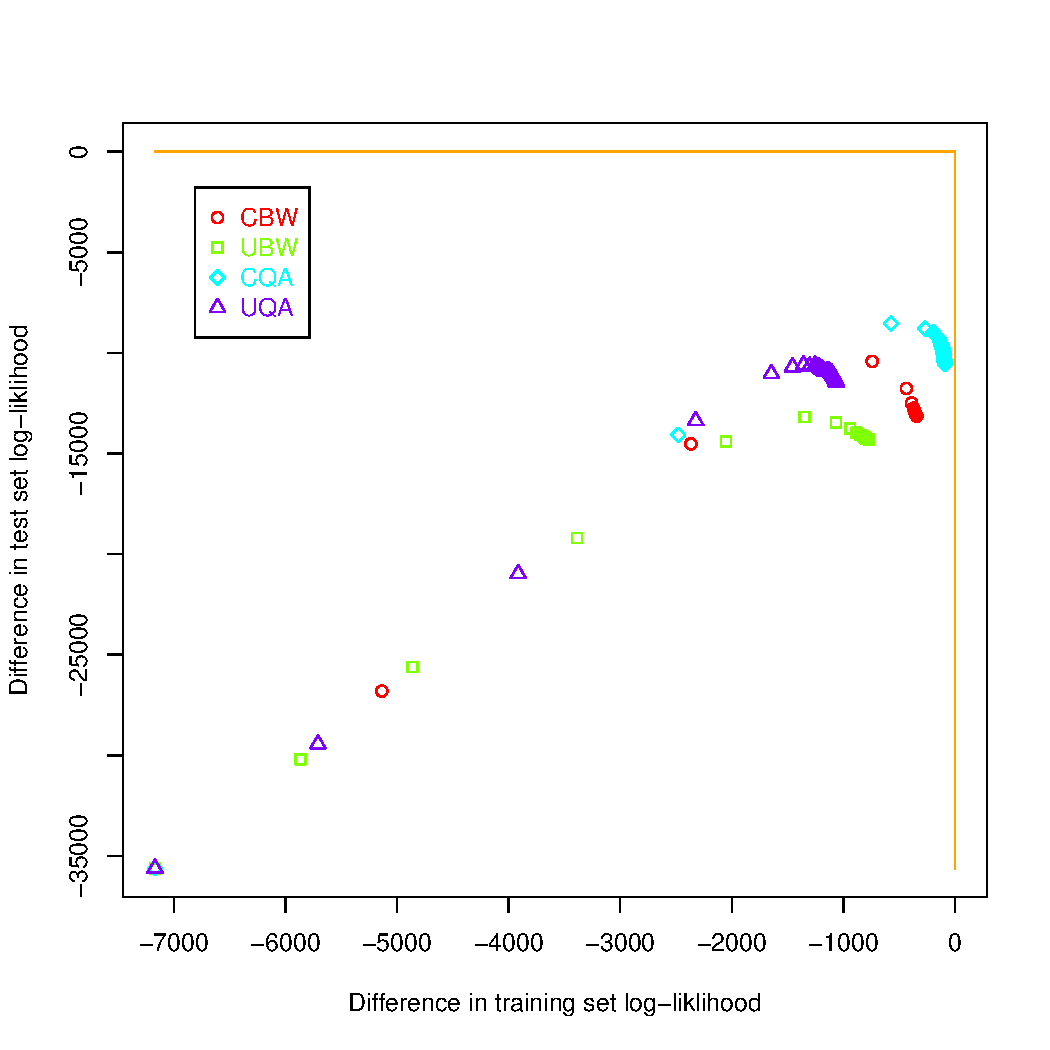
\includegraphics[scale=.85]{DNA_uniformstart_results_90.pdf}
\caption{\textbf{DNA Simulation Results for Concentration Rate 0.90, starting from concentrated uniform positions.}  DNA results for the scenario with 20 sequences drawn from a profile of length 1000 for a conservation rate of $0.90$ are shown, color coded by method.  The points plot the iterations of the algorithm from 0 to convergence, from left to right.  The X axis shows the difference in the $\log_{10}$ likelihood of the training set data, and the Y axis shows the difference in the test set data, with differences taken to the true model from which the data were drawn.  Starting from uniform positions appears to trap all of the algorithms in local optima.}.
\label{fig:DNA_uniformstart_results_90}
\end{figure}


%Figure~\ref{cbw_fig:dnaTrainingResults} depicts the average log-probabilities of the training sets for the 16 runs at each conservation level for the DNA Profile HMM study.  Figure~\ref{cbw_fig:dnaTestResults} depicts the average log-probabilities of the test sets.  Figures \ref{cbw_fig:proteinTrainingResults} and  \ref{cbw_fig:proteinTestResults} show the results for the protein study.

% \begin{figure}[!htp]
% \centering
% %\subfigure[average log-probabilities of the DNA training data]{\label{cbw_fig:dnaTrainingTable}\centering\includegraphics[scale=.3]{simulationDNATrainingForwardTable.pdf}} \\
% %\subfigure[graph of (a), with values shifted to be non-negative]{\label{cbw_fig:dnaTrainingGraph}\centering\includegraphics[scale=.2625]{simulationDNATrainingForwardGraph.pdf}} \\
% % \caption{\textbf{DNA training data simulation results.} Each row in (a) and set of bars in (b) corresponds to a different conservation level in the 4 ``true profiles''.  The first column and the top bar (white) depicts the average log-probability of the training sequences using the 16 starting profiles.  The second (amber) depicts the average log-probability of the training sequences using the true profiles.  The third (red) depicts the average log-probability using the Baum-Welch (BW) algorithm.  The fourth (blue) depicts the average log-probability using the Conditional Baum-Welch (CBW) algorithm.  All bars in (b) have been shifted so that the lowest bar is at 0.  The CBW algorithm outperforms BW at conservation levels above .6.  At .5 and below, CBW does not outperform BW.}
%  \label{cbw_fig:dnaTrainingResults}
% \end{figure}
% 
% \begin{figure}[!htp]
% \centering
% \subfigure[average log-probabilities of the DNA test data]{\label{cbw_fig:dnaTestTable}\centering\includegraphics[scale=.3]{simulationDNATestForwardTable.pdf}} \\
% \subfigure[graph of (a), with values shifted to be non-negative]{\label{cbw_fig:dnaTestGraph}\centering\includegraphics[scale=.2625]{simulationDNATestForwardGraph.pdf}} \\
%  \caption{\textbf{DNA test data simulation results.} Data are represented as in Figure~\ref{cbw_fig:dnaTrainingResults}.  As in the training data results in Figure~\ref{cbw_fig:dnaTrainingResults}, the new algorithm outperforms BW at conservation levels above .6.}
%   \label{cbw_fig:dnaTestResults}
% \end{figure}
% 
% \begin{figure}[!htp]
% \centering
% \subfigure[average log-probabilities of the protein training data]{\label{cbw_fig:proteinTrainingTable}\centering\includegraphics[scale=.3]{simulationProteinTrainingForwardTable.pdf}} \\
% \subfigure[graph of (a), with values shifted to be non-negative]{\label{cbw_fig:proteinTrainingGraph}\centering\includegraphics[scale=.2625]{simulationProteinTrainingForwardGraph.pdf}} \\
%  \caption{\textbf{Protein training data simulation results.} Data are represented as in Figure~\ref{cbw_fig:dnaTrainingResults}.  The CBW algorithm outperforms BW at every conservation level.}
%   \label{cbw_fig:proteinTrainingResults}
% \end{figure}
% 
% \begin{figure}[!htp]
% \centering
% \subfigure[average log-probabilities of the protein test data]{\label{cbw_fig:proteinTestTable}\centering\includegraphics[scale=.3]{simulationProteinTestForwardTable.pdf}} \\
% \subfigure[graph of (a), with values shifted to be non-negative]{\label{cbw_fig:proteinTestGraph}\centering\includegraphics[scale=.2625]{simulationProteinTestForwardGraph.pdf}} \\
%  \caption{\textbf{Protein test data simulation results.} Data are represented as in Figure~\ref{cbw_fig:dnaTrainingResults}.  As in the training data results in Figure~\ref{cbw_fig:proteinTrainingResults}, these results show the CBW algorithm outperforming BW at every conservation level.}
%   \label{cbw_fig:proteinTestResults}
% \end{figure}

\subsection{HIV-1 Founder Identification}
A Profile HMM represents sequences that are independent and identically distributed, which may be appropriate for endogenous and exogenous viruses that evolve with little phylogenetic structure, such as transposons and RNA virus families \citep[sequence weighting strategies to account for subfamily structure have been proposed; see][]{Durbin}. Here we discuss its application to the modeling of subpopulations of HIV-1 \textit{in vivo}.  During acute HIV-1 infection (in the first few weeks post-acquisition), HIV-1 viruses replicate at a high rate. Due to the low fidelity replication mechanism of HIV-1, new errors are introduced with each replication cycle.  The sequences diversify primarily in a manner described well by a Poisson distribution \citep{Giorgi:2010aa}, with little linkage across sites, because constant recombination among a ``quasispecies cloud'' of viral particles limits linkage \citep{Neher1509.02483v1,Wu:2014aa}.  This results in a sequence distribution that is well represented by a Profile HMM.  However, in some fraction of infections there are multiple distinguishable founders of infection; estimates range from 20-30\% of infections and vary by exposure route \citep{Gounder:2015aa, Sterrett:2014aa, Li:2010aa, Gottlieb:2008aa}.  For some time these populations evolve independently, each with its own star-like phylogeny.  Methods have been proposed for evaluating the impact of preventative vaccination by accounting for a possible reduction in the number of founders, rather than simply evaluating the binary endpoint of acquisition \citep{FollmannMultiplicityVE}. Furthermore, the evaluation of so-called ``acquisition sieve effects'' (indication of a genome-specific effect of the vaccine to prevent infection against some but not all HIV-1 viruses) requires reconstruction of the founding viruses \citep{edlefsen2013sieve}. Determining the number of founders is an important part of vaccine evaluation, and several authors have described methods for counting founders using a combination of automated and manual evaluation techniques \citep{Keele:2008aa,Herbeck:2011aa,Rossenkhan:2012aa}, though no fully automated (and hence reproducible) method has yet been described.

Here we evaluate a simple approach to estimating HIV-1 infection founder multiplicity that leverages a unique feature of Profile HMMs that have been estimated using the techniques described here (that is, maximum likelihood or maximum a posteriori parameters): at convergence, the Baum-Welch update vectors for each participant mutually cancel \citep{PaulsPosterAtHIVDynamics2015}.  This property is guaranteed for all of the methods evaluated here, even the (C)QA methods because at convergence the gradient of the log-likelihood is zero, and \cite{Baldi:1994} showed that this gradient is also the gradient of the Baum-Welch EM Q function.  The per-sequence Baum-Welch update vectors are the conditional expected values of the PHMM's parameters, given that the model produced just that sequence, and so these have the same structure as the Profile HMM.

We call these per-sequence update vectors ``alignment profiles'' as they represent averages over all possible paths through the latent states of the model, which corresponds to all of the ways to align the sequence to the model.  Under the \textit{iid} assumptions of the PHMM, these alignment profiles should be uncorrelated vectors.  Violations of the assumption are reflected in unexpected clustering among the vectors, and here we use this insight to implement a method for counting the number of founders, and ultimately for modeling each founder quasispecies population as a separate PHMM.

Our approach is straightforward, and is meant to demonstrate the utility of true statistical estimation of PHMM parameters rather than to be a final solution to the founder identification problem.  For each subject's set of (unaligned) sampled sequences, we estimate the parameters of a Profile HMM using CQA.  We use this Profile HMM to estimate one alignment profile per sequence.  We cluster these vectors (by performing UPGMA clustering on the matrix of Euclidean distances between them) and then cut the tree using the ``Dynamic Tree Cut'' method of \cite{Langfelder01032008}, using default options.  The first cut is at a height of it 99\% of the range between the 5th percentile and the maximum of the joining heights on the dendrogram, regardless of the heterogeneity of the sequences, and will thus always result in at least two clusters.  To accept a call of greater than 1 founder we also require a minimum PHMM entropy (summed over the PHMM) of 20. This is a Profile HMM analogue of the requirement of a minimum sequence diversity commonly applied in the founder identification literature, but differs in that the entropy of the PHMM accounts for alignment uncertainty.


The LANL HIV sequence database \citep[url: ][]{LANL} provides curated ``special purpose'' nucleotide alignments of HIV-1 sampled from acute infections, including a set of 1505 HIV-1 Clade C env nucleotide sequences collected from 69 patients \citep[described in][]{Abrahams:2009aa}. We follow the authors' suggestion to pre-filter the sequences to exclude any found to have signatures of ``hypermutation'', a well-described effect of a human anti-viral mechanism \citep[we use][]{rose2000detecting} or recombination \citep[using RAPBeta, url:][]{RAPBeta}. We prepare the sequences by stripping the gaps (unaligning them).  We evaluate our ability to detect founders by comparing our estimated number of founders for each subject against those calculated by the study's authors.

Tables~\ref{tbl:AbrahamsFoundersVsProfillicFounders-a},~\ref{tbl:AbrahamsFoundersVsProfillicFounders-b},~and~\ref{tbl:AbrahamsFoundersVsProfillicFounders-c} show the results of this experiment, indicating that in this case the automated founder detection works quite well. The tables show, for each of the 69 participants studied, the time at which their acute infection was sampled \citep[as Fiebig stages][]{fiebig2003dynamics}, the number of sequences sampled, the number of these sequences excluded because they were found to have hypermutation or recombination, and the statistics computed after Profillic HMM analysis.  The final two columns show the comparison of the reported number of founders from our analysis and those of the original study.  The Profillic HMM statistics are the ``entropy'', which is actually the sum of entropy values over all of the PHMM parameters after parameter estimation using the default parameter options of the Profillic implementation of CQA for DNA sequence families, and the number of clusters obtained from the clustering of update vectors.

\begin{table}
\centering
\begin{tabular}{cc | ccc | cc | cc}
  \hline
Participant & Fiebig & nSeq & nHyper & nRcmb & Pent & Pclst & Ours & Theirs \\ 
  \hline
0089 &  5 &  22 &   0 &   0 & 6.76 &   3 & 1 &   1 \\ 
  0114 &  4 &  27 &   0 &   4 & 65.50 &   3 & 3 &   3 \\ 
  0334 &  1-2 &  22 &   0 &   0 & 5.02 &   2 & 1 &   1 \\ 
  0393 &  4 &  22 &   0 &   0 & 5.57 &   2 & 1 &   1 \\ 
  0478 &  1-2 &  23 &   0 &   3 & 70.71 &   2 & 2 &   3 \\ 
  0595 &  4 &  28 &   0 &   0 & 6.93 &   6 & 1 &   1 \\ 
  0626 &  4 &  24 &   0 &   0 & 5.57 &   2 & 1 &   1 \\ 
  0665 &  4 &  20 &   0 &   0 & 6.86 &   2 & 1 &   1 \\ 
  0682 &  1-2 &  22 &   0 &   0 & 4.73 &   2 & 1 &   1 \\ 
  0985 &  1-2 &  23 &   0 &   0 & 4.61 &   2 & 1 &   1 \\ 
  1086 &  1-2 &  24 &   0 &   0 & 8.49 &   2 & 1 &   1 \\ 
  1172 &  1-2 &  20 &   0 &   0 & 4.90 &   2 & 1 &   1 \\ 
  1176 &  1-2 &  21 &   0 &   0 & 9.27 &   3 & 1 &   3 \\ 
  1196 &  1-2 &  23 &   2 &   0 & 32.78 &   2 & 2 &   3 \\ 
  1335 &  4 &  21 &   0 &   1 & 85.85 &   2 & 2 &   3 \\ 
  1373 &  1-2 &  22 &   0 &   0 & 6.36 &   3 & 1 &   1 \\ 
  1394 &  1-2 &  20 &   0 &   0 & 6.40 &   3 & 1 &   1 \\ 
  2010 &  4 &  23 &   0 &   0 & 6.78 &   2 & 1 &   1 \\ 
  2052 &  1-2 &  23 &   0 &   0 & 5.46 &   2 & 1 &   1 \\ 
  2060 &  1-2 &  22 &   0 &   0 & 5.55 &   2 & 1 &   1 \\ 
  2103 &  1-2 &  20 &   0 &   0 & 4.83 &   2 & 1 &   1 \\ 
   \hline
\end{tabular}
\caption{\textbf{Profillic Founder Identification Using CQA: Table 1 of 3}}
\label{tbl:AbrahamsFoundersVsProfillicFounders-a}
\end{table}

\begin{table}
\centering
\begin{tabular}{cc | ccc | cc | cc}
  \hline
Participant & Fiebig & nSeq & nHyper & nRcmb & Pent & Pclst & Ours & Theirs \\ 
  \hline
  703010010 &  2 &  22 &   0 &   0 & 21.40 &   3 & 3 &   3 \\ 
  703010054 &  5-6 &  27 &   0 &   0 & 15.91 &   2 & 1 &   1 \\ 
  703010131 &  4 &  22 &   0 &   0 & 6.10 &   2 & 1 &   1 \\ 
  703010159 &  2 &  20 &   0 &   0 & 6.89 &   5 & 1 &   1 \\ 
  703010193 &  4 &  24 &   1 &   0 & 6.75 &   2 & 1 &   1 \\ 
  703010200 &  4 &  18 &   0 &   8 & 57.09 &   3 & 3 &   3 \\ 
  703010217 &  5-6 &  25 &   0 &   0 & 6.63 &   2 & 1 &   1 \\ 
  703010228 &  4 &  28 &   0 &   3 & 53.28 &   2 & 2 &   2 \\ 
  704010017 &  5-6 &  25 &   0 &   0 & 14.24 &   3 & 1 &   1 \\ 
  704010042 &  4 &  42 &   0 &   0 & 7.80 &   2 & 1 &   1 \\ 
  704010056 &  5-6 &  21 &   0 &   1 & 17.73 &   4 & 1 &   1 \\ 
  704010069 &  4 &  23 &   0 &   0 & 9.71 &   2 & 1 &   1 \\ 
  704010083 &  2 &  24 &   0 &   0 & 6.15 &   2 & 1 &   1 \\ 
  704809221 &  1-2 &  28 &   0 &   0 & 6.85 &   2 & 1 &   1 \\ 
  704810053 &  1-2 &  20 &   0 &   0 & 7.61 &   2 & 1 &   1 \\ 
  704810015 &  x &  23 &   0 &   0 & 9.84 &   3 & 1 &   1 \\ 
  705010026 &  x &  23 &   0 &   0 & 7.79 &   3 & 1 &   1 \\ 
  705010078 &  4 &  26 &   0 &   0 & 5.99 &   3 & 1 &   1 \\ 
  705010110 &  x &  20 &   0 &   0 & 8.98 &   6 & 1 &   1 \\ 
  706010018 &  4 &  23 &   0 &   0 & 15.52 &   2 & 1 &   1 \\ 
  706010151 &  6 &  15 &   0 &   7 & 53.90 &   2 & 2 &   2 \\ 
  706010164 &  4 &  19 &   0 &   0 & 5.23 &   2 & 1 &   1 \\ 
   \hline
\end{tabular}
\caption{\textbf{Profillic Founder Identification Using CQA: Table 2 of 3}}
\label{tbl:AbrahamsFoundersVsProfillicFounders-b}
\end{table}
 

\begin{table}
\centering
\begin{tabular}{cc | ccc | cc | cc}
  \hline
Participant & Fiebig & nSeq & nHyper & nRcmb & Pent & Pclst & Ours & Theirs \\ 
  \hline
  CAP129 &  4 &  19 &   0 &   0 & 5.20 &   2 & 1 &   1 \\ 
  CAP136 &  5 &  16 &   0 &   2 & 28.86 &   2 & 2 &   2 \\ 
  CAP174 &  5 &  21 &   0 &   0 & 6.37 &   2 & 1 &   1 \\ 
  CAP177 &  1-2 &  20 &   0 &   0 & 4.97 &   2 & 1 &   1 \\ 
  CAP188 &  1-2 &  22 &   0 &   0 & 5.51 &   2 & 1 &   1 \\ 
  CAP200 &  5 &  18 &   0 &   0 & 5.77 &   2 & 1 &   1 \\ 
  CAP206 &  5 &  21 &   0 &   0 & 6.30 &   2 & 1 &   1 \\ 
  CAP210 &  1-2 &  21 &   0 &   0 & 4.35 &   2 & 1 &   1 \\ 
  CAP217 &  5 &  20 &   0 &   0 & 4.88 &   2 & 1 &   1 \\ 
  CAP220 &  1-2 &  15 &   0 &   0 & 7.61 &   2 & 1 &   1 \\ 
  CAP221 &  1-2 &  21 &   0 &   0 & 7.10 &   2 & 1 &   1 \\ 
  CAP222 &  1-2 &  21 &   0 &   0 & 54.08 &   3 & 3 &   3 \\ 
  CAP224 &  5 &  19 &   0 &   0 & 21.18 &   2 & 2 &   2 \\ 
  CAP225 &  3 &  20 &   0 &   0 & 6.85 &   2 & 1 &   1 \\ 
  CAP237 &  3 &  22 &   0 &   0 & 5.87 &   2 & 1 &   1 \\ 
  CAP239 &  5 &  24 &   0 &   0 & 6.49 &   3 & 1 &   1 \\ 
  CAP260 &  5 &  18 &   0 &   5 & 47.68 &   2 & 2 &   2 \\ 
  CAP269 &  6 &  18 &   0 &   0 & 16.37 &   3 & 1 &   1 \\ 
  CAP37 &  4 &  20 &   0 &   2 & 67.29 &   3 & 3 &   3 \\ 
  CAP40 &  6 &  22 &   1 &   0 & 12.04 &   2 & 1 &   1 \\ 
  CAP45 &  1-2 &  16 &   0 &   0 & 4.81 &   2 & 1 &   1 \\ 
  CAP63 &  3 &  19 &   1 &   0 & 5.93 &   2 & 1 &   1 \\ 
  CAP69 &  1-2 &  20 &   0 &   9 & 61.61 &   3 & 3 &   5 \\ 
  CAP8  &  5 &  62 &   0 &   1 & 13.93 &   3 & 1 &   1 \\ 
  CAP84 &  4 &  22 &   1 &   0 & 5.67 &   1 & 1 &   1 \\ 
  CAP85 &  6 &  21 &   2 &   0 & 11.89 &   2 & 1 &   1 \\ 
   \hline
\end{tabular}
\caption{\textbf{Profillic Founder Identification Using CQA: Table 3 of 3}}
\label{tbl:AbrahamsFoundersVsProfillicFounders-c}
\end{table}

\section{Discussion}
Here we have presented a new algorithm for estimating the parameters of a Profile HMM. While a related method was previously proposed \citep{baldi1994smooth}, we describe an efficient procedure for calculation of the step size parameter, which is necessary for deployment of the approach. We show the first evidence of comparable performance as compared with the Baum-Welch algorithm and its conditional variant.  We also show that the same ``rotated'' orientation to the algorithm allows for a conditional ascent procedure yields advantages over unconditional maximization, consistent with what was shown previously for Conditional Baum-Welch \citep{edlefsen2010transposon}.  Through simulation studies we have shown that new algorithm, Conditional Quadratic Ascent, performs comparably in most scenarios to CBW, however its performance in large-sequence, low sample size settings demonstrates an improvement over that method.

\begin{figure}
\centering
\includegraphics[scale=.8]{abrahams-2009aa-results_phmm_entropy_hist.pdf}
\caption{\textbf{Histogram of Profile HMM entropy values.} These are the sum of individual entropy values over individual multinomial distributions for the parameters of the PHMM, and are thus model-length-dependent.  The value of 20 gave the best agreement with the results of \cite{Abrahams:2009aa}.}
\label{fig:PHMM_entropy_hist}
\end{figure}

The Profile Hidden Markov model represents a good candidate model for within-host HIV-1 sequence diversity within a single quasispecies cloud, because such clouds of constantly recombining variants are expected to be distributed as approximately independent representatives from a plateau in the fitness landscape \citep{Domingo01012002,vignuzzi2006quasispecies}.  Here we have demonstrated a property of true maximization of the parameters of a PHMM when the \textit{iid} assumption holds: at convergence, the update vectors cancel and are expected to be independent and identically distributed.  We introduced the notion of clustering these ``alignment profiles'' to detect violations from \textit{iid}, and we showed that this can be productively applied to the important scientific aim of identifying distinct viral founder populations in acute HIV-1 infection.

The results of our simple method agreed with the founder multiplicity in most instances.  Apart from participant ``1176'', using a threshold of PHMM entropy of 20 classified the participants into single and multiple founder variants in agreement with those of \cite{Abrahams:2009aa}.  The authors noted that this participant had an ``infection with 3 closely related viruses,'' perhaps explaining the relatively low entropy.  We chose the value 20 to optimize agreement with their method; as Figure~\ref{fig:PHMM_entropy_hist} shows, this represents one of multiple gaps in the distribution.  However, these entropy values are not scaled for the length of the model (which here was around 2500 positions), and further work is needed to determine a general strategy for setting this threshold from the data alone, ideally one that is robust to variations in HIV-1 clade, Fiebig stage, model length and genomic region. Among the remaining 14 participants that were identified by both methods as multiple-founder variants, there was agreement on 10. In the simple analysis we conducted, the remaining four participants were assigned lower estimates by our method (by one in three cases: two instead of three; and by two in the case of CAP69: three instead of five).  It turns out that for CAP69, two of the five ``founders'' were unique recombinants of the other three founders  (C. Williamson, personal communication). Thus that particular discrepancy is due to the fact that we removed recombinants before conducting our analysis.  All four of these participants' viral populations exhibited recombination or hypervariation, so the other discrepancies may have the same source, or may simply be due to the relatively simple method that we used for clustering.  Further work is needed to develop the method into a full-fledged automated procedure for HIV-1 founder identification.

\section{Acknowledgments}
The author gratefully acknowledges the early contributions to the development of this method by Andrew F. Siegel, Eugene Kolker, and Robert Hubley.

Research reported in this publication was supported by the National Institute Of Allergy And Infectious Diseases (NIAID) of the National Institutes of Health (NIH) under Award Numbers R37AI054165 and UM1AI068635, and by the Bill and Melinda Gates Foundation Award Number OPP1110049. The content is solely the responsibility of the authors and does not necessarily represent the official views of the NIH or BMGF.

%% The Appendices part is started with the command \appendix;
%% appendix sections are then done as normal sections
%% \appendix

%% \section{}
%% \label{}

%% If you have bibdatabase file and want bibtex to generate the
%% bibitems, please use
%%
\bibliographystyle{elsarticle-harv} 
\bibliography{CQAPaper}

%%% ERE I AM
%% Warning--I didn't find a database entry for "TravissBenchmarksPaper"
%% Warning--I didn't find a database entry for "LANLS_aligner"
%% Warning--I didn't find a database entry for "SimonsAligner"
%% Warning--I didn't find a database entry for "LANLonAlignmentsOrSomething"
%% Warning--I didn't find a database entry for "Giorgi:2010aa"
%% Warning--I didn't find a database entry for "Herbeck:2011aa"
%% Warning--I didn't find a database entry for "Rossenkhan:2012aa"
%% Warning--I didn't find a database entry for "PaulsPosterAtHIVDynamics"
%% Warning--I didn't find a database entry for "LANL"
%% Warning--I didn't find a database entry for "HYPERMUT"
%% Warning--I didn't find a database entry for "RAPBeta"


% %% else use the following coding to input the bibitems directly in the
% %% TeX file.
% 
% \begin{thebibliography}{00}
% 
% %% \bibitem[Author(year)]{label}
% %% Text of bibliographic item
% 
% \bibitem[ ()]{}
% 
% \end{thebibliography}

\end{document}

\endinput
%%
%% End of file `elsarticle-template-harv.tex'.
